\documentclass[10pt]{article}

\usepackage{tikz}
\usepackage{tkz-euclide}
%\usetkzobj{all}

\usepackage{blindtext}
\usepackage{nccmath}
\usepackage{commath}
\usepackage{parskip}
\usepackage{siunitx}
\usepackage{titlesec}
\usepackage[dvipsnames]{xcolor}
\usepackage[utf8]{inputenc}
\usepackage[T1]{fontenc}
\usepackage{float}
\usepackage{graphicx}
%\usepackage[left=2cm right=2cm top=2cm bottom=2cm]{geometry}
\usepackage{textcomp}
\usepackage{geometry}
\usepackage{enumerate}
\usepackage{layout}
\usepackage{ulem}
\usepackage{amsmath}
\usepackage{tikz}
\usepackage{forest,adjustbox}
\usepackage{subcaption}
\usepackage{caption}
\usetikzlibrary{decorations.markings}
\usetikzlibrary{patterns}
\usepackage{amsfonts}
\usepackage{amssymb}
\usepackage{chemfig}
\usepackage{chemist}
\usepackage[version=4]{mhchem}
\usepackage{chemfig}
\usepackage{color}
\usepackage{mathtools}
\usepackage{textgreek}
\usepackage{amssymb}
\usetikzlibrary{shapes}
\usetikzlibrary{arrows}
\usepackage{pgfplots}
\pgfplotsset{width=10cm,compat=1.9}
\usepgfplotslibrary{external}
%\usepackage[table]{xcolor}
\usepackage{colortbl,hhline}
\usepackage{newunicodechar}
\usepackage{fourier}
\usepackage{rotating}
\usepackage[latin9]{inputenc}
\usepackage{amssymb}
%\usetikzlibrary{arrows}
%\usepackage{tikz-3dplot-circleofsphere}
\usetikzlibrary{quotes, angles}
%\usepackage{pgf}
\usetikzlibrary{patterns}
%\usetikzlibrary{calc,perspective}

\geometry{a4paper, left=10mm, right=10mm, top=10mm, bottom=20mm}

\usepackage{fancyhdr, lastpage}
\pagestyle{fancy}
\fancyfoot[C]{{\thepage} / \pageref{LastPage}}
\usepackage{rotating}

\newcommand\logeq{\mathrel{\vcentcolon\Leftrightarrow}}

\begin{document}

\textbf{Larget-Piet Julien} \\

Made with LaTeX

%\hspace{\fill} LaTeX

\vspace*{2cm}

\Huge

\begin{center}

        \textbf{Automatisation sur Diagramme Ternaire à $\mathbf{n}$ variables}\\[0.5cm]

\end{center}

\normalsize

\vspace{1.5cm}

\hspace{1cm} Bien que ce document prend pour exemple le point de mélange (proportion massique d'un mélange de plusieurs composés), la demonstration peut aussi convenir dans d'autres cas où des équations de modélisation sont présentes. \\

\hspace{1cm} Ce document est la documentation technique du programme libre et en source ouverte (License: MIT) se trouvant à l'addresse suivante: \textbf{https://github.com/iro0087/...} permettant de visualiser des diagrammes ternaires de manière \textbf{interractive}. \\

\hspace{1cm} Le code source de ce document LaTeX se retrouve dans le dépot Git à l'addresse précédente. \\

\vspace{3cm}

\hspace{0cm}\begin{tikzpicture}

        \put(162.35,14.85){\rotatebox{0}{\draw (0,0) coordinate (A)  
                                -- (8,0) coordinate (C) 
                                -- (4,8) coordinate (B) 

                  -- cycle;}}

        \put(162.35,14.85){\rotatebox{0}{\draw (0,0) coordinate (A) 
                                -- (2,0) coordinate (C)
                                -- (1,2) coordinate (B)

                  -- cycle;}}

\end{tikzpicture}

\newpage

\newcommand\kitty{\leavemode\xleaders\hbox{.}\hfill\kern0pt\vspace{0.15cm}}

\begin{center}

        \Large \textbf{SOMMAIRE} \normalsize

\end{center}

\vspace{1cm}

\begin{itemize}

        \item Introduction \kitty (3 - 5) 

        \hspace{1cm} - Propriétés \kitty (3 - 4)

        \hspace{1cm} - Objectif \kitty (5)

        \item  Détermination des fonctions proportion de chaque variable \kitty (6 - 7) 

        \hspace{1cm} - $p_{B}$ \kitty (6) 

        \hspace{1cm} - $p_{C}$ \kitty (6) 

        \hspace{1cm} - $p_{A}$ \kitty (7) 

        \item Déduction des fonctions graduation de chaque variable \kitty (7 - 14) 

        \hspace{1cm} - $p_{B}$ \kitty (7 - 10) 

        \hspace{2cm} - Déduction de la fonctions perpendiculaire à la fonction graduation de $p_{B}$ \kitty (7 - 8) 

        \hspace{2cm} - $P_{B}$ - $1^{ère}$ situation $(180 - \color{blue}g_{B}\color{black}) < 90$ \kitty (8 - 9) 

        \hspace{2cm} $P_{B}$ - $2^{ème}$ situation $(180 - \color{blue}g_{B}\color{black}) > 90$ \kitty (9 - 10) 
        
        \hspace{1cm} - $p_{C}$ \kitty (10 - 12) 

        \hspace{2cm} - Déduction des fonctions perpendiculaires à la fonction graduation de $p_{C}$ \kitty (10)

        \hspace{2cm} - $P_{C}$ - $1^{ère}$ situation $(180 - \color{red}g_{C}\color{black}) < 90$ \kitty (11 - 12) 

        \hspace{2cm} - $P_{C}$ - $2^{ème}$ situation $(180 - \color{red}g_{C}\color{black}) > 90$ \kitty (12) 

        \hspace{1cm} - $p_{A}$ \kitty (12 - 14)

        \hspace{2cm} - Déduction des fonctions perpendiculaires à la fonction graduation de $p_{A}$ \kitty (12 - 13)

        \hspace{2cm} - $P_{A}$ - $1^{ère}$ situation $(180 - \color{orange}g_{C}\color{black}) < 90$ \kitty (13) 

        \hspace{2cm} - $P_{A}$ - $2^{ème}$ situation $(180 - \color{orange}g_{C}\color{black}) > 90$ \kitty (14) 

        \item Application pour $n$ variables \kitty (15 - 18) 

        \hspace{1cm} - Présentation \kitty (15 - 18)

        \hspace{2cm} - Cas de l'égalité des coefficients \kitty (16)

        \hspace{1cm} - Exemple pour 8 variables \kitty (18)

        \item Conclusion \kitty (19) 

\end{itemize}

\normalsize

\newpage

\vspace{1cm}

\normalsize

\uline{\textbf{Introduction:}}

\vspace{.5cm}

\uline{Propriétés:}

\vspace{.5cm}
\begin{minipage}{.43\textwidth}

        \begin{itemize}

        \item Un diagramme ternaire est un triangle \textbf{équilatéral}.\\[.25cm]

        \item Chaque angle fait donc $\frac{180}{3}$ = \textbf{60°}\\[.25cm]

        \item Les propportions des variables $\color{blue}\textbf{B}\color{black}$, $\color{red}\textbf{C}\color{black}$ et $\color{orange}\textbf{A}\color{black}$ seront respectivement notées comme $\color{blue}\mathbf{{p}_{B}}\color{black}$, $\color{red}\mathbf{{p}_{C}}$ et $\color{orange} \mathbf{{p}_{A}} \color{black}$ \\[.25cm]

        Dans le cas d'un mélange, $p_{B;A;C} \in [0;\mathbf{\frac{1}{3}}]$ \\[1cm]

        \end{itemize}

\end{minipage}%
\hspace{4cm}\begin{minipage}{.66\textwidth}%
        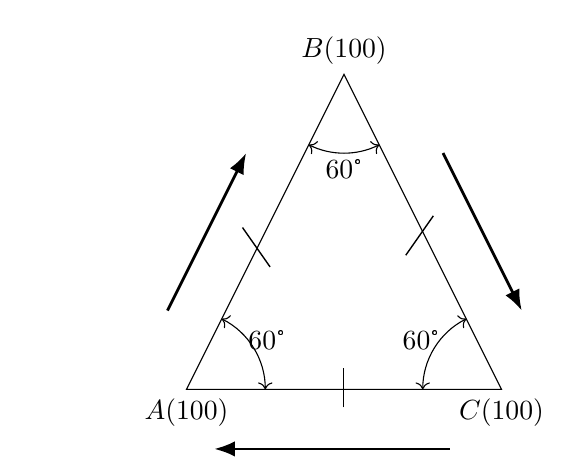
\begin{tikzpicture}

                \draw (0,0) coordinate (A) node[anchor=north] {$A (100)$}
                  -- (4,0) coordinate (C) node[anchor=north] {$C (100)$}
                  -- (2,4) coordinate (B) node[anchor=south] {$B (100)$}
                  pic["60°", draw=black, <->, angle eccentricity=1.2, angle radius=1cm]
                {angle=A--B--C}
                
                  pic["60°", draw=black, <->, angle eccentricity=1.2, angle radius=1cm]
                {angle=C--A--B}
                
                  pic["60°", draw=black, <->, angle eccentricity=1.2, angle radius=1cm]
                {angle=B--C--A}

                  -- cycle;

                \put(10, -50){\draw [line width=1pt, arrows = {Latex-[length=0pt 3 0]}] (0,1) -- (3,1);}

                \put(50,0){\draw [line width=1pt, arrows = {Latex-[length=0pt 0 3]}] (-1,3) -- (-2,1);}

                \put(50, 0){\draw [line width=1pt, arrows = {Latex-[length=0pt 3 0]}] (2.5,1) -- (1.5,3);}

                \put(42.5, -35){\draw [line width=.5pt] (.5, 1) -- (.5, 1.5);}

                \put(65, 20){\draw [line width=.5pt] (.5, 1) -- (0.85, 1.5);}

                \put(6, 30){\draw [line width=.5pt] (.5, 1) -- (0.85, .5);}

        \end{tikzpicture}

\end{minipage}%

\vspace{1cm}

Pour la suite les angles \color{orange}$g_{A}$,\color{black} $\color{blue}g_{B}$ et $\color{red}g_{C}$ correspondront à cela: \\

\hspace{3cm}\begin{minipage}{.43\textwidth}
\begin{tikzpicture}

        %base

        \put(50,-100){\draw (0,0) coordinate (A) node[anchor=north] {$A$}
                  -- (2,0) coordinate (C) 
                  -- (1,2) coordinate (B)

                  pic["\color{orange}$180 - g_{A}$\color{black}", draw=black, <->, angle eccentricity=1.2, angle radius=1cm]
                {angle=B--C--A}

          -- cycle;}

          \put(106,-100){\draw (0,0) coordinate (A) 
                  -- (2,0) coordinate (C) 
                  -- (1,2) coordinate (B)

          -- cycle;}

          \put(162,-100){\draw (0,0) coordinate (A) 
                          -- (2,0) coordinate (C) node [anchor=north] {$C$} 
                  -- (1,2) coordinate (B)

                  pic["\color{red}$180 - g_{C}$\color{black}", draw=back, <->, angle eccentricity=1.2, angle radius=1cm]
                  {angle=A--B--C} 

          -- cycle;}

        %second floor


          \put(135,-43){\rotatebox{180}{\draw (0,0) coordinate (A) 
                  -- (2,0) coordinate (C) 
                  -- (1,2) coordinate (B)

                  -- cycle;}}

        \put(191,-43){\rotatebox{180}{\draw (0,0) coordinate (A) 
                  -- (2,0) coordinate (C) 
                  -- (1,2) coordinate (B)

                  -- cycle;}}

        %third floor


        \put(133,-43){\rotatebox{0}{\draw (0,0) coordinate (A) 
                  -- (2,0) coordinate (C) 
                  -- (1,2) coordinate (B)

                  -- cycle;}}


        \put(78,-43){\rotatebox{0}{\draw (0,0) coordinate (A) 
                  -- (2,0) coordinate (C) 
                  -- (1,2) coordinate (B)

                  -- cycle;}}

        \put(162.35,14.85){\rotatebox{180}{\draw (0,0) coordinate (A) 
                  -- (2,0) coordinate (C) 
                  -- (1,2) coordinate (B)

                  -- cycle;}}

        %top
         
        \put(106,15){\rotatebox{0}{\draw (0,0) coordinate (A) 
                  -- (2,0) coordinate (C) 
                  -- (1,2) coordinate (B) node[anchor=south] {$B$}

                  pic["$\color{blue}180 - g_{B}$\color{black}", draw=black, <->, angle eccentricity=1.2, angle radius=1cm]
                {angle=C--A--B}

                  -- cycle;}}


          \put(71, -90){\draw [line width=1pt, orange] (.255, 1.66) -- (1.255, -.35);}

          \put(70, -90){\draw [line width=1.1pt, red] (3.25, -.35) -- (4.25, 1.66);}

          \put(99, -32.5){\draw [line width=1pt, blue] (.255, 1.66) -- (2.25, 1.66);}

        \put(90, -150){\draw [line width=1pt, arrows = {Latex-[length=0pt 3 0]}] (0,1) -- (3,1);}

        \put(110,-70){\draw [line width=1pt, arrows = {Latex-[length=0pt 0 3]}] (-1,3) -- (-2,1);}

        \put(140, -70){\draw [line width=1pt, arrows = {Latex-[length=0pt 3 0]}] (2.5,1) -- (1.5,3);}

        \end{tikzpicture}
\end{minipage}%

\vspace{4cm}

\hspace{7cm}Diagramme ternaire à 2 graduations.

\vspace{1.5cm}

\begin{itemize}

        \item La graduation de chaque variable se remarque en identifiant la première ligne partant de la plus grande proportion graduée de cette dernière. \\[.125cm]

        \item Il y a une infinité de graduations car une infinité de proportion existe pour chaque variable. \\[.5cm]

\end{itemize}

\newpage

\vspace*{1cm}

\begin{itemize}

        \item Un diagramme ternaire peut être non-linéare, c'est à dire que les graduations d'une proportion de variable peuvent \textbf{ne pas être parallèles entre elles}. \\[1cm]

\end{itemize}

\hspace{0cm}\begin{tikzpicture}

        \put(162.35,14.85){\rotatebox{0}{\draw (0,0) coordinate (A) node [anchor=north] {A} 
                                -- (8,0) coordinate (C) node [anchor=north] {C}
                                -- (4,8) coordinate (B) node [anchor=south] {B}

                  -- cycle;}}

        \put(0, -28.5){\draw [line width=.5pt, dotted] (7,1.52) -- (9.7,9.5);}

        \put(0, -28.5){\draw [line width=.5pt, dotted] (12,1.52) -- (9.7,9.5);}

        \put(0, -28.5){\draw [line width=.5pt, dotted] (9.7,1.52) -- (9.7,9.5);}

\end{tikzpicture}

\begin{center}

        \color{red}\danger\color{black} Pour des questions de visibilité, seule $p_{A}$ a été représentée

\end{center}

\vspace{1cm}

\begin{itemize}

        \item $\color{blue}g_{B}\color{black}$, $\color{red}g_{B}\color{black}$ et $\color{orange}g_{A}\color{black}$ seront les angles des graduations \textbf{pour une proportion donnée}.

\end{itemize}

\vspace{1cm}

\color{purple}\begin{tabular}{| c |}

        \hline

        \textbf{Le problème revient à déduire les fonctions graduation d'au moins 2 variables afin d'en déduire le point d'intersection.} \\ \hline

\end{tabular}
\color{black}

\vspace{1cm}

\begin{center}

        \Large $\color{blue}F_{B}\color{black} = \color{red}F_{C}\color{black} = \color{orange}F_{A}\color{black}$ \normalsize

\end{center}

\newpage

\uline{Objectif:}

\vspace{.5cm}

\begin{itemize}

        \item Un diagramme ternaire nous permet de savoir quel mélange faire pour avoir certaines propriétés qu'on voit avec des équations de modélisation dont les réponses $R_{n}$ sont représentées ci-sessous:

\end{itemize}

\vspace{2cm}

\centerline{\begin{minipage}{1.05\textwidth}

\begin{tikzpicture}

        \put(162.35,14.85){\rotatebox{0}{\draw (0,0) coordinate (A) node [anchor=north] {A} 
                                -- (8,0) coordinate (C) node [anchor=north] {C}
                                -- (4,8) coordinate (B) node [anchor=south] {B}

                  -- cycle;}}

                  \put(162.35,14.85){\rotatebox{0}{\draw[color=blue, fill, opaque] (0,0) coordinate (A)  
                                -- (3,0) coordinate (C)
                                -- (1.5,3) coordinate (B) 

                  -- cycle;}}

                  \put(162.35,14.85){\rotatebox{0}{\draw[color=blue, fill, opaque] 

                  plot [smooth cycle] coordinates {(1.5,3) (3,2) (3,0)}
                  
                  -- cycle;}}

                  %\put(247.4, 15) {\rotatebox{-63}{\draw[color=blue, fill, semitransparent] (0,0) arc (0:180:1.67cm and .75cm);}}

                  \put(233.5,156){\rotatebox{0}{\draw[color=red, fill, opaque] (0,0) coordinate (A)  
                                -- (3,0) coordinate (C) 
                                -- (1.5,3) coordinate (B) 

                  -- cycle;}}

                  \put(233.5,156){\rotatebox{0}{\draw[color=red, fill, opaque] 

                  plot [smooth cycle] coordinates {(0,0) (1.5,-1) (3,0)}
                  
                  -- cycle;}}

                  %\put(233.5, 156.3) {\rotatebox{180}{\draw[color=red, fill, semitransparent] (0,0) arc (0:180:1.5cm and .75cm);}}


                  \put(305,14.85){\rotatebox{0}{\draw[color=orange, fill, opaque] (0,0) coordinate (A)  
                                -- (3,0) coordinate (C) 
                                -- (1.5,3) coordinate (B) 

                  -- cycle;}}

                  \put(305,14.85){\rotatebox{0}{\draw[color=orange, fill, opaque] 

                  plot [smooth cycle] coordinates {(0,0) (-.15,2) (1.5,3)}
                  
                  -- cycle;}}

                  %\put(349, 100) {\rotatebox{63}{\draw[color=orange, fill, semitransparent] (0,0) arc (0:180:1.7cm and .75cm);}}


                  \draw (7,1.5) node {\huge $\color{white}R_{1}\color{black}$ \normalsize}

                  \draw (12,1.5) node {\huge $\color{white}R_{3}\color{black}$ \normalsize}

                  \draw (9.7,6.7) node {\huge $\color{white}R_{2}\color{black}$ \normalsize}

                  \draw (9.7,3.5) node {\huge $R_{4}$ \normalsize}

\end{tikzpicture}

\end{minipage}}

\begin{itemize}

        \item Différentes équationd de modélisation peuvent être utilisées qui prennent plus ou moins les interractions entre chaque paramètre, avec $a_{n}$ des constantes:

\end{itemize}

\vspace{2cm}

- $R = a_{0} + a_{1}\cdot \color{blue}p_{B}\color{black} + a_{2}\cdot \color{red}p_{C}\color{black} + a_{3}\cdot \color{orange}p_{A}\color{black}$, chaque variable est indépendante \\

- $R = a_{0} + a_{1}\cdot \color{blue}p_{B}\color{black} + a_{2}\cdot \color{red}p_{C}\color{black} + a_{3}\cdot \color{orange}p_{A}\color{black} + a_{1;2}\cdot \color{blue}p_{B}\color{black}\cdot \color{red}p_{C}\color{black} + a_{1;3}\cdot \color{blue}p_{B}\color{black}\cdot \color{orange}p_{A}\color{black} + a_{2;3}\cdot \color{red}p_{C}\color{black}\cdot \color{orange}p_{A}\color{black}$, l'intrraction deux à deux entre variable est prise en compte \\

- $R = a_{0} + a_{1}\cdot \color{blue}p_{B}\color{black} + a_{2}\cdot \color{red}p_{C}\color{black} + a_{3}\cdot \color{orange}p_{A}\color{black} + a_{1;2}\cdot \color{blue}p_{B}\color{black}\cdot \color{red}p_{C}\color{black} + a_{1;3}\cdot \color{blue}p_{B}\color{black}\cdot \color{orange}p_{A}\color{black} + a_{2;3}\cdot \color{red}p_{C}\color{black}\cdot \color{orange}p_{A}\color{black} + a_{1;2;3}\cdot \color{blue}p_{B}\color{black}\cdot \color{red}p_{C}\color{black}\cdot \color{orange}p_{A}\color{black}$, l'intrraction deux à deux entre variable est prise en compte \\

- Ce sont les \textbf{couleurs} qui informent l'utilisateur de la Réponse

\vspace{2cm}


\color{red}\danger\color{black} On a représenté les équations de modélisation pour 3 variables mais on peut le faire pour $\mathbf{n}$ variables.


%\begin{center}

%        \includegraphics[scale=0.4]{model.jpg}

%\end{center}

%\newpage

%\uline{Pré-requis:}

%\vspace{1cm}

%\begin{itemize}

%        \item Pour des questions de lisibilité des équations, nous passerons des coordonnées d'un repère à l'autre comme décrit ci-dessous:

%\end{itemize}

%\vspace{.5cm}

%\begin{minipage}{.5\textwidth}
        
%\hspace{2cm}\begin{tikzpicture}

%\put(0, -28.5){\draw [line width=1pt, arrows = {Latex-[length=0pt 3 0]}] (4.1,1) -- (0,1);}

%\put(0, -28.5){\draw [line width=1pt, arrows = {Latex-[length=0pt 3 0]}] (0,5) -- (0,1);}

%\put(0, -28.5){\draw [line width=1pt, color=purple] (1.5,1) -- (1.5,2.8);}

%\draw (1.5,2) node {P}

%\draw (0, 5) node {\textbf{A}}

%\draw (-0.5,0) node {O}

%\end{tikzpicture}
%\end{minipage}%
%\begin{minipage}{.5\textwidth}

%\hspace{1cm}\begin{turn}{-30}\begin{tikzpicture}

%\put(0, -28.5){\draw [line width=1pt, arrows = {Latex-[length=0pt 3 0]}] (4.1,1) -- (0,1);}

%\put(0, -28.5){\draw [line width=1pt, arrows = {Latex-[length=0pt 3 0]}] (0,5) -- (0,1);}

%\put(0, -28.5){\draw [line width=1pt, color=purple] (1.5,1) -- (1.5,2.8);}

%\draw (1.5,2) node {P'}

%\put(-70,60) {\rotatebox{-70}{\draw[<->, bend right=45, line width = 1pt] (1,1) to  (4,1);}}

%\draw (-1.8, 0) node {\rotatebox{30}{$30$°}}

%\draw (0, 5) node {\rotatebox{30}{\textbf{B}}}

%\draw (-0.5,0) node {O}

%\end{tikzpicture}
%\end{turn}
%\end{minipage}

%\begin{itemize}

%        \item On cherche à déterminer $x_{P'}$ et $y_{P'}$ dans le repère \textbf{A} si on superposait les repères.

%\end{itemize}

%\vspace{.5cm}

%\begin{tikzpicture}



%\end{tikzpicture}

\newpage

\uline{\textbf{Détermination des fonctions proportion de chaque variable:}}

\vspace{2.5cm}

\begin{minipage}{.43\textwidth}

        \vspace{.5cm}

        \hspace{.5cm} \uline{Pour $p_{B}$:} \\[.125cm]

        \begin{itemize}

                \item On a donc 2 points et donc une droite, mais aussi une fonction :) \\[.25cm]

                \item C'est une fonction affine passant par A(0;0) et S d'équation: \\[.125cm]

                        \hspace{2cm} $Y_{B}$ = $\frac{y_{S} - y{A}}{x_{S} - x_{A}}x$ = $\frac{1}{0.5}x$ = $2x$, $\forall x \in [0; \textbf{0.5}]$ \\[.25cm]


        \item Comme on est dans un triangle équilatéral: Si, $p_{B} = 0.6$ \Leftrightarrow $x_{P} = 0.6 \cdot \textbf{0.5} = 0.3$ \\[.25cm]

        \item Les coordonnées de ce point P seront: \\[.25cm]

                \hspace{1cm} P(0.3;$Y_{B}(0.3)$) \Leftrightarrow  P(0.3;$2\mathbind{\cdot}0.3$) \Leftrightarrow P (0.3;0.6) 

        \end{itemize}

\end{minipage}%
\hspace{5cm}\begin{minipage}{.66\textwidth}
        \begin{tikzpicture}

                \draw (0,0) node[anchor=north]
                  -- (4,0) node[anchor=north]
                  -- (2,4) node[anchor=south]{$S$}
                  -- cycle;

          \draw [thick, blue] (0,0)  -- (1.1, 2.2) node[anchor=west]{$P$}; 

          \draw (1.12, 2) node[anchor=south]{\rotatebox{-45}{+}} 

          \draw (-.5, -.5) node {\color{red}(0;0)}

                \draw (-.5, 4) node {(0;1)}

                \draw (5, -.5) node {(1;0)}

                \draw (3, 4) node {\color{red}(0.5;1)}

                \draw (2.125, 2.125) node {\color{blue}(0.3;0.6)}

                \put(0, -28.5){\draw [line width=1pt, arrows = {Latex-[length=0pt 3 0]}] (4.1,1) -- (0,1);}
     
                \put(0, -28.5){\draw [line width=1pt, arrows = {Latex-[length=0pt 3 0]}] (0,5) -- (0,1);}

        \end{tikzpicture}

\end{minipage}%

\vspace{3cm}

\begin{minipage}{.43\textwidth}

        \hspace{.5cm} \uline{Pour $p_{C}$:} \\[.125cm]

        \begin{itemize}

                \item C'est une fonction affine passant par C(1;0) et S: \\[.125cm]

                        \hspace{.5cm} $a_{C}$ = $\frac{y_{C} - y_{S}}{x_{C} - x_{S}}x$ = $\frac{-1}{0.5}x$ = $-2x$ \\[.25cm]


                        \hspace{.5cm} $Y_{C}(1) = 0 \Leftrightarrow -2\cdot 1 + b = 0$ \Leftrightarrow $b = 2$ \\[.25cm]

                        \hspace{1.5cm} $Y_{C} = -2x + 2$, $\forall x \in [\textbf{0.5};1]$ \\[.25cm]

        \end{itemize}

        \begin{itemize}

                \item Si $p_{C} = 0.4$, les coordonnées de ce point P seront: \\[.125cm]

                $x_{P} = \textbf{0.5} + \textbf{0.5}\cdot 0.4 = 0.7$ \\[.125cm]

                P(0.7;$Y_{B}(0.7)$) \Leftrightarrow  P(0.8;$-2\mathbind{\cdot}0.7 + 2$) \Leftrightarrow P (0.7;0.6) 

        \end{itemize}

\end{minipage}%
\hspace{5cm}\begin{minipage}{.66\textwidth}
        \begin{tikzpicture}

                \draw (0,0) node[anchor=north]
                  -- (4,0) node[anchor=north]
                  -- (2,4) node[anchor=south]{$S$}
                  -- cycle;

          \draw [thick, blue] (4,0)  -- (2.9, 2.2) node[anchor=west]{$P$}; 

          \draw (2.9, 2) node[anchor=south]{\rotatebox{-45}{+}} 

          \draw (-.5, -.5) node {(0;0)}

          \draw (-.5, 4) node {(0;1)}

          \draw (5, -.5) node {\color{red}(1;0)}

                  \draw (3, 4) node {\color{red}(\textbf{0.5};1)}

          \draw (4.125, 2.125) node {\color{blue}(0.7;0.6)}

          \put(0, 0){\draw [line width=1pt, dotted] (2,0) -- (2,4);}

          \put(0, -28.5){\draw [line width=1pt, arrows = {Latex-[length=0pt 3 0]}] (4.1,1) -- (0,1);}

          \put(0, -28.5){\draw [line width=1pt, arrows = {Latex-[length=0pt 3 0]}] (0,5) -- (0,1);}

          \end{tikzpicture}

\end{minipage}%

\newpage

\begin{minipage}{.43\textwidth}

        \hspace{.5cm} \uline{Pour $p_{A}$:} \\[.125cm]

        \begin{itemize}

                \item On peut associer $p_{A}$ à un repère en une dimension avec un sens inversé. \\[.25cm]

        \end{itemize}

        \begin{itemize}

                \item Si $p_{A} = 0.75$, les coordonnées de ce point P seront: \\[.125cm]

                $x_{P} = 1 - 0.75 = 0.25$ \\[.125cm]

                P(0.75;0)

        \end{itemize}

\end{minipage}%
\hspace{5cm}\begin{minipage}{.66\textwidth}

        \vspace{2.5cm}

        \begin{tikzpicture}

                \draw (0,0) node[anchor=north]
                  -- (4,0) node[anchor=north]
                  -- (2,4) node[anchor=south]
                  -- cycle;

          \draw (.9, -.23) node[anchor=south]{\rotatebox{-45}{+}} 

          \draw (1.2, 6.05) node[anchor=south]{\rotatebox{-45}{+}} 

          \draw (1.2, 6.25) node[anchor=south]{$p_{A} = 0.75$} 

          \draw (-.5, -.5) node {\color{red}(0;0)}

          \draw (-.5, 4) node {(0;1)}

          \draw (5, -.5) node {\color{red}(1;0)}

          \draw (.9, -.6) node {\color{blue}(0.25;0)}

          \put(0, 150){\draw [line width=1pt, arrows = {Latex-[length=0pt 3 0]}] (0,1) -- (4.1,1);}

          \put(0, -28.5){\draw [line width=1pt, arrows = {Latex-[length=0pt 3 0]}] (4.1,1) -- (0,1);}

          \put(0, -28.5){\draw [line width=1pt, arrows = {Latex-[length=0pt 3 0]}] (0,5) -- (0,1);}

          \draw [line width = 1.1pt, blue] (4,0)  -- (.9, 0) node[anchor=north]{$P$}; 

          \end{tikzpicture}

\end{minipage}%

\uline{\textbf{Déduction des fonctions graduation de chaque variable:}} \\[.5cm]

\begin{center}

       \Large \uline{Pour $p_{B}$} \normalsize  \\

\end{center}

\begin{itemize}

        \item On cherche les fonctions donnant des droites perpendiculaires à [A,B]:

\end{itemize}

\begin{center}

\begin{minipage}{.66\textwidth}
\begin{tikzpicture}

                \draw (0,0) node[anchor=north]
                  -- (4,0) node[anchor=north]
                  -- (2,4) node[anchor=south]{$S$}
                  -- cycle;

          \draw (2, 6) node {Si P(0.25;0.5),}

          \draw (-.5, -.5) node {(0;0)}

          \draw (-.5, 4) node {(0;1)}

          \draw (5, -.5) node {(1;0)}

          \draw (3, 4) node {(0.5;1)}

                  \draw (1.3, 0.5) node {\color{red}$\Delta_{1}$}

                  \draw (1.6, -0.3) node {\color{red}$\Delta_{2}$}

          \draw (.7, 1.8) node[anchor=south]{P} 

          \draw (.9, 1.6) node[anchor=south]{\rotatebox{45}{+}} 

          \put(0, -28.5){\draw [line width=1pt, arrows = {Latex-[length=0pt 3 0]}] (4.1,1) -- (0,1);}

          \put(0, -28.5){\draw [line width=1pt, red, dotted] (3.8,1) -- (0.9,1);}

          \put(0, -28.5){\draw [line width=1pt, arrows = {Latex-[length=0pt 3 0]}] (0,5) -- (0,1);}

          %\put(0, -28.5){\draw [line width=1pt] (0,0) -- (4,-3);}

          \put(25,50){\rotatebox{-115}{\draw (0,.5)-|(.5,0);}}

          \put(0, -28.5){\draw [line width=1pt] (.9,2.85) -- (4,1);}

          \put(0, -28.5){\color{red}\draw [line width=1pt, dotted] (.9,2.85) -- (.9,1);}

          \draw (4.25, 0) node {P'}

          \put(-31, 24){\color{red}\draw [line width=1pt, dotted] (1.1,1) -- (2,1);}

\end{tikzpicture}
\end{minipage}%
\begin{minipage}{.66\textwidth}

\begin{tikzpicture}

        \draw (0,0) node[anchor=north]
                  -- (4,0) node[anchor=north]
                  -- (2,4) node[anchor=south]{$S$}
                  -- cycle;

          \draw (-.5, -.5) node {(0;0)}

          \draw (2, 5) node {Pour un point P quelconque,}

          \draw (-.5, 4) node {(0;1)}

          \draw (5, -.5) node {(1;0)}

          \draw (3, 4) node {(0.5;1)}

          \put(0, -28.5){\draw [line width=1pt, arrows = {Latex-[length=0pt 3 0]}] (4.1,1) -- (0,1);}

          \put(0, -28.5){\draw [line width=1pt, arrows = {Latex-[length=0pt 3 0]}] (0,5) -- (0,1);}

          %\put(0, -28.5){\draw [line width=1pt] (0,0) -- (4,-3);}

          \put(28,25){\rotatebox{-210}{\draw (.5,0)-|(0,.5);}}

          \draw (0.3, .7) node[anchor=south]{P} 

          \draw (0.37, .5) node[anchor=south]{\rotatebox{45}{+}} 

          \put(-15, -61.5){\draw [line width=1pt] (.9,2.85) -- (4,1);}

          \put(0, -61.5){\draw [line width=1pt, red, dotted] (3.45,1) -- (.35,1);}

          \put(-15, -61.5){\color{red}\draw [line width=1pt, dotted] (.9,2.85) -- (.9,1);}

          \draw (.7, -.5) node {\color{red}$\Delta_{1}$}

          \draw (1.2, -1.5) node {\color{red}$\Delta_{2}$}

          \draw (3.9, -1.1) node {P'}

          \draw (3.45, -1.15) node {\rotatebox{45}{+}}

          %\put(-15, -61.5){\color{red}\draw [line width=1pt, dotted] (.9,1) -- (2,1);}

\end{tikzpicture}

\end{minipage}

\end{center}

\vspace{1cm}

\begin{itemize}

        \item Tous les segments perpendiculaires à une même droite sont parallèles entre eux.

        \item On en déduit que pour chaque point de [A,B], la droite perpendiculaire peut être décrite comme une fonction affine: \\

\end{itemize}

\color{red}\danger\color{black} $\Delta_{1}$ ainsi que $\Delta_{2}$ sont des valeurs absolues. Pour des questions de praticité, car eles vont être réutilisées.\\

\end{center}

                $\alpha = \frac{y_{P'} - y_{P}}{x_{P'} - x_{P}}x \Leftrightarrow \frac{\Delta_{1}}{\Delta_{2}}$ \\

        $\frac{\Delta_{1}}{\Delta_{2}}\cdot (x_{P} + \Delta2) + b = y_{P} - \Delta_{1}$ \Leftrightarrow  $b = Y_{B}(x_{P}) - \Delta_{1} - \frac{\Delta_{1}}{\Delta_{2}}\cdot (x_{P} + \Delta_{2}) \Leftrightarrow b = 2x_{P} - \Delta_{1} - \frac{\Delta_{1}}{\Delta_{2}}\cdot (x_{P} + \Delta_{2})}\Leftrightarrow b = 2\cdot0.5\cdot p_{B} - \Delta_{1} - \frac{\Delta_{1}}{\Delta_{2}}\cdot (0.5\cdot p_{B} + \Delta_{2})$ 

\newpage

\vspace{1cm}

\begin{center}

        \begin{itemize}

                \item Pour trouver $\Delta_{1}$ et $\Delta_{2}$, on prend une situation particulière: \\[.5cm]

        \end{itemize}

        P(0.25;0.5) \Rightarrow P'(1;0) \\[.5cm]

        \begin{cases}
      
                x_{P} + \Delta{2} = x_{P'} \\
      
                y_{P} - \Delta_{1} = y_{P'}
    
        \end{cases} \Leftrightarrow
        \begin{cases}
      
                \Delta_{2} = x_{P'} - x_{P} \\
      
                \Delta_{1} = y_{P'} - y_{P}

        \end{cases} \Leftrightarrow
        \begin{cases}

                \color{red}\Delta_{2} \color{black} = \abs{1 - 0.25} = \color{red} 0.75 \color{black} \\ 

                \color{red} \Delta_{1} \color{black} = \abs{0 - 0.5} = \color{red} 0.5 \color{black}

        \end{cases}

\end{center}

\begin{center}

        $\color{blue}Y_{p_{B}}\color{black} = ax + b \Leftrightarrow \color{blue}Y_{P_{B}}\color{black} = \color{red} - \color{black}\alpha x + b$ \\[.25cm]

$\color{blue}Y_{p_{B}}\color{black} = -\frac{\Delta_{1}}{\Delta_{2}}x + 2\cdot 0.5\cdot p_{B} - \Delta_{1} - \frac{\Delta_{1}}{\Delta_{2}}\cdot (0.5\cdot p_{B} + \Delta_{2})}$ \\[.25cm]

$\color{blue}Y_{p_{B}}\color{black} = -\frac{0.5}{0.75}x + 2\cdot 0.5\cdot p_{B} - 0.5 - \frac{0.5}{0.75}\cdot (0.5\cdot p_{B} + 0.75), \forall x \in \mathbb{R}$

\end{center} 

\vspace{.25cm}

\begin{itemize}

        \item On cherche les fonctions des graduations de $p_{B}$:

\end{itemize}

\uline{$180 - \color{blue}g_{B}\color{black} < 90$:}

\begin{minipage}{.66\textwidth}
\begin{tikzpicture}

                \draw (0,0) node[anchor=north]
                  -- (4,0) node[anchor=north]
                  -- (2,4) node[anchor=south]{$S$}
                  -- cycle;

          \draw (-.5, -.5) node {(0;0)}

          \draw (-.5, 4) node {(0;1)}

          \draw (5, -.5) node {(1;0)}

          \draw (3, 4) node {(0.5;1)}

          \draw (.7, 1.7) node[anchor=south]{P} 

          \draw (.9, 1.6) node[anchor=south]{\rotatebox{45}{+}} 

          \put(0, -28.5){\draw [line width=1pt, arrows = {Latex-[length=0pt 3 0]}] (4.1,1) -- (0,1);}

          \put(0, -28.5){\draw [line width=1pt, arrows = {Latex-[length=0pt 3 0]}] (0,5) -- (0,1);}

          %\put(0, -28.5){\draw [line width=1pt] (0,0) -- (4,-3);}

          \put(25,51){\rotatebox{-115}{\draw (0,.5)-|(.5,0);}}

          \put(0, -28.5){\draw [line width=1pt, color=purple] (.9,2.85) -- (2,2.18);}

          \put(0, -28.5){\draw [line width=1pt] (.9,2.85) -- (2.1,3.1);}

          \draw (2.25, 1) node {P'}

          \draw (2.35, 2.3) node {P''}

          \put(20, 71) {\draw[color=blue] (.6,-.6) arc (0:80:.3cm);}

          \put(59, 49) {\rotatebox{230}{\draw[color=teal] (.6,-.6) arc (90:130:.38cm);}}

          \draw (1.4,2) node[anchor=south] {\color{blue}$180 - g_{B}$} 

          \draw (1.8,1.5) node[anchor=south] {\color{teal}$g_{P}$} 

\end{tikzpicture}
\end{minipage}%
\centerline{\begin{minipage}{1.4\textwidth}

                \begin{turn}{15}\begin{tikzpicture}

        \put (-10,59) {\rotatebox{141}{\draw [line width=1pt] (.6,-.6) arc (0:360:2.5cm);}}

        \put(55, -45){\draw [line width=1pt, arrows = {Latex-[length=0pt 3 0]}] (1.3,4.8) -- (-2.05,1.02);}

        %\put(55, -45){\draw [line width=1pt] (-0.55,2.75) -- (-2.05,1.02);}

        \put(55, 27){\draw [line width=1pt, arrows = {Latex-[length=0pt 3 0]}] (1.4,-1.33) -- (-2.3,2.1);}

                \put(55, 27){\rotatebox{-15}{\draw [line width=.7pt, dotted] (-0.5,2.75) -- (-0.5,-2.25);}}

        \put(77, 15) {\rotatebox{200}{\draw[color=teal] (.6,-.6) arc (90:180:.3cm);}}

        \draw (2.6,.7) node[anchor=south] {\color{teal}$g_{P}$} 

        \put(55, -45){\draw [line width=1pt] (-.4,2.85) -- (2.1,3);}

        \put(55, -45){\draw [line width=1pt, dotted] (.81,4.3) -- (2.1,3);}

        \put(55, -45){\draw [line width=1pt, dotted] (.9,1.7) -- (2.1,3);}

        \draw (3.8, -1) node[anchor=south] {$cos(x)$}

        \draw (4.8, 1.2) node[anchor=south] {$P''$}

        \draw (3.1, 1.5) node[anchor=south] {\color{purple}$\delta_{p''} = rayon$}

        \draw (-1, 2.7) node[anchor=south] {$\pi$}

        \draw (4.2, 3) node[anchor=south] {$sin(x)$}

        %\draw (-.8, -1) node[anchor=south] {$sin(x)$}

\end{tikzpicture}

\end{turn}

\end{minipage}}

\begin{center}

$\color{blue}180 - g_{B}\color{black} + 90 + \color{teal}g_{P}\color{black} = 180 \Leftrightarrow \color{teal}g_{P}\color{black} = -\left(90 - \color{blue}g_{B}\color{black}\right)$°

\end{center}

\begin{itemize}

        \item On prend arbitrairement $\color{purple}\delta_{P''}\color{black} = \color{purple}0.2\color{black}$ \\[.25cm]

        \item On en déduit les équations suivantes:

\end{itemize}

\vspace{1cm}

\begin{center}

        \begin{cases}

                x_{P''} = x_{P'} - \left(\color{purple}\delta_{P''}\color{black} - cos\left(\frac{\color{teal}g_{P}}{180}\pi\right)\cdot \color{purple}\delta_{P''}\color{black}\right) \\

                y_{P''} = y_{P'} + \left(sin\left(\frac{\color{teal}g_{P}}{180}\pi\right)\cdot \color{purple}\delta_{P''}\color{black}\right)

        \end{cases}

        \Leftrightarrow

        \begin{cases}

                x_{P''} = (x_{P} - \color{purple}0.2\color{black}) + \left(\color{purple}0.2\color{black} - cos\left(\frac{\color{teal}g_{P}}{180}\pi\right)\cdot \color{purple}0.2\color{black}\right) \\

                y_{P''} = Y_{p_{B}}(x_{P} + \color{purple}0.2\color{black}) + \left(sin\left(\frac{\color{teal}g_{P}}{180}\pi\right)\cdot \color{purple}0.2\color{black}\right)

        \end{cases}

        \Leftrightarrow

        \begin{cases}

                x_{P''} = (x_{P} - \color{purple}0.2\color{black}) + \left(\color{purple}0.2\color{black} - cos\left(\frac{-(\color{teal}90 - g_{B}\color{black})}{180}\pi\right)\cdot \color{purple}0.2\color{black}\right) \\

                y_{P''} = -\frac{0.5}{0.75}\cdot \left(x_{P} + \color{purple}0.2\color{black}\right) + 2\cdot x_{P} - 0.5 - \frac{0.5}{0.75}\cdot (x_{P} + 0.75)  + \left(sin\left(\frac{-(\color{teal}90 - g_{B})}{180}\pi\right)\cdot \color{purple}0.2\color{black}\right)

        \end{cases}

        \newpage %page5

        \Leftrightarrow

        \begin{cases}

                x_{P''} = (p_{B}\cdot 0.5 - \color{purple}0.2\color{black}) + \left(\color{purple}0.2\color{black} - cos\left(\frac{-(\color{teal}90 - g_{B})}{180}\pi\right)\cdot \color{purple}0.2\color{black}\right) \\

                y_{P''} = -\frac{0.5}{0.75}\cdot (p_{B}\cdot 0.5 + \color{purple}0.2\color{black}) + 2\cdot (p_{B}\cdot 0.5) - 0.5 - \frac{0.5}{0.75}\cdot ((p_{B}\cdot 0.5) + 0.75)  + \left(sin\left(\frac{-(\color{teal}90 - g_{B})}{180}\pi\right)\cdot \color{purple}0.2\color{black}\right)

        \end{cases}

\end{center}

\vspace{.5cm}

\begin{itemize}

        \item On en déduit la ou les fonctions représentants les graduations de $p_{B}$: \\[.25cm]

\end{itemize}

\begin{center}

        $a = \frac{y_{P''} - y_{P}}{x_{P''} - x_{P}} \Leftrightarrow a = \frac{-\frac{0.5}{0.75}\cdot (p_{B}\cdot 0.5 + \color{purple}0.2\color{black}) + 2\cdot (p_{B}\cdot 0.5) - 0.5 - \frac{0.5}{0.75}\cdot ((p_{B}\cdot 0.5) + 0.75)  + \left(sin\left(\frac{-(\color{teal}90 - g_{B})}{180}\pi\right)\cdot \color{purple}0.2\color{black}\right)
        - (2\cdot p_{B}\cdot 0.5)
}{(p_{B}\cdot 0.5 + \color{purple}0.2\color{black}) - \left(\color{purple}0.2\color{black} - cos\left(\frac{-(\color{teal}90 - g_{B})}{180}\pi\right)\cdot \color{purple}0.2\color{black}\right) - (p_{B}\cdot 0.5)}$ \\[.25cm]

%$a\cdot (x_{P} + 0.2) + b = y_{P''} \Leftrightarrow b = y_{P''} - a\cdot (x_{P} + 0.2) \Leftrightarrow b = \frac{-0.5}{0.75}x +2\cdot (p_{B}\cdot 0.5 + 0.2) - 0.5 - \frac{0.5}{0.75}\cdot ((p_{B}\cdot 0.5 + 0.2) + 0.75)  + sin(\frac{\color{teal}g_{P}}{180}\pi\cdot \color{purple}\delta_{P''}\color{black}) - \frac{\frac{-0.5}{0.75}x +2\cdot (p_{B}\cdot 0.5 + 0.2) - 0.5 - \frac{0.5}{0.75}\cdot ((p_{B}\cdot 0.5 + 0.2) + 0.75)  + sin(\frac{\color{teal}g_{P}}{180}\pi\cdot \color{purple}\delta_{P''}\color{black})
 %- \frac{-0.5}{0.75}x +2\cdot p_{B}\cdot 0.5 - 0.5 - \frac{0.5}{0.75}\cdot (p_{B}\cdot 0.5 + 0.75)
%}{(p_{B}\cdot 0.5 + 0.2) + (\color{purple}\delta_{P''}\color{black} - cos(\frac{\color{teal}g_{P}}{180}\pi)\cdot \color{purple}\delta_{P''}\color{black}) - p_{B}\cdot 0.5}\cdot (p_{B}\cdot 0.5 + 0.2)$

$a\cdot x_{P} + b = y_{P} \Leftrightarrow b = y_{P} - a\cdot x_{P}$ \\[.25cm]

$\Leftrightarrow b = 2\cdot (p_{B}\cdot 0.5) - \frac{-\frac{0.5}{0.75}\cdot (p_{B}\cdot 0.5 + \color{purple}0.2\color{black}) + 2\cdot (p_{B}\cdot 0.5) - 0.5 - \frac{0.5}{0.75}\cdot ((p_{B}\cdot 0.5) + 0.75)  + \left(sin\left(\frac{-(\color{teal}90 - g_{B})}{180}\pi\right)\cdot \color{purple}0.2\color{black}\right)
        -(2\cdot p_{B}\cdot 0.5)
}{(p_{B}\cdot 0.5 + \color{purple}0.2\color{black}) - \left(\color{purple}0.2\color{black} - cos\left(\frac{\color{teal}-(90  - g_{B})}{180}\pi\right)\cdot \color{purple}0.2\color{black}\right) - (p_{B}\cdot 0.5)}\cdot (p_{B}\cdot 0.5)$ \\[.25cm]

$\color{blue}F_{p_{B}}\color{black} = \frac{-\frac{0.5}{0.75}\cdot (p_{B}\cdot 0.5 + \color{purple}0.2\color{black}) + 2\cdot (p_{B}\cdot 0.5) - 0.5 - \frac{0.5}{0.75}\cdot ((p_{B}\cdot 0.5) + 0.75)  + \left(sin\left(\frac{-(\color{teal}90 - g_{B})}{180}\pi\right)\cdot \color{purple}0.2\color{black}\right)
        - (2\cdot p_{B}\cdot 0.5)
}{(p_{B}\cdot 0.5 + \color{purple}0.2\color{black}) - \left(\color{purple}0.2\color{black} - cos\left(\frac{-(\color{teal}90 - g_{B})}{180}\pi\right)\cdot \color{purple}0.2\color{black}\right) - (p_{B}\cdot 0.5)}x\\[.25cm]

+ 2\cdot (p_{B}\cdot 0.5) - \frac{-\frac{0.5}{0.75}\cdot (p_{B}\cdot 0.5 + \color{purple}0.2\color{black}) + 2\cdot (p_{B}\cdot 0.5) - 0.5 - \frac{0.5}{0.75}\cdot ((p_{B}\cdot 0.5) + 0.75)  + \left(sin\left(\frac{-(\color{teal}90 - g_{B})}{180}\pi\right)\cdot \color{purple}0.2\color{black}\right)
        -(2\cdot p_{B}\cdot 0.5)
}{(p_{B}\cdot 0.5 + \color{purple}0.2\color{black}) - \left(\color{purple}0.2\color{black} - cos\left(\frac{-(\color{teal}90 - g_{B})}{180}\pi\right)\cdot \color{purple}0.2\color{black}\right) - (p_{B}\cdot 0.5)}\cdot (p_{B}\cdot 0.5)$ \\[.25cm]

\vspace{.25cm}

\forall x \in \mathbb{R}

\end{center}

\vspace{1cm}

\begin{itemize}

        \item L'utilisateur n'a qu'à renseigner le proportion de la variable B ainsi que l'angle de sa graduation et la fonction graduation de B sera établie 
        \item On fait de même pour les autres situations

\end{itemize}

\vspace{.5cm}

\uline{$180 - \color{blue}g_{B}\color{black} > 90$:}

\begin{minipage}{.66\textwidth}
\begin{tikzpicture}

                \draw (0,0) node[anchor=north]
                  -- (4,0) node[anchor=north]
                  -- (2,4) node[anchor=south]{$S$}
                  -- cycle;

          \draw (-.5, -.5) node {(0;0)}

          \draw (-.5, 4) node {(0;1)}

          \draw (5, -.5) node {(1;0)}

          \draw (3, 4) node {(0.5;1)}

          \draw (.7, 1.9) node[anchor=south]{P} 

          %\draw (.35, 1.3) node[anchor=south]{22.5°} 

          \draw (.9, 1.6) node[anchor=south]{\rotatebox{45}{+}} 

          \put(0, -28.5){\draw [line width=1pt, arrows = {Latex-[length=0pt 3 0]}] (4.1,1) -- (0,1);}

          \put(0, -28.5){\draw [line width=1pt, arrows = {Latex-[length=0pt 3 0]}] (0,5) -- (0,1);}

          %\put(0, -28.5){\draw [line width=1pt] (0,0) -- (4,-3);}

          \put(25,51){\rotatebox{-385}{\draw (0,.5)-|(.5,0);}}

          \put(0, -28.5){\draw [line width=1pt] (.9,2.85) -- (2,2.18);}

          \put(0, -28.5){\draw [line width=1pt] (.9,2.85) -- (1.7,1.7);}

          \draw (2.25, 1) node {P'}

          \draw (2, 1.22) node {\rotatebox{45}{+}}

          \draw (2, .6) node {P''}

          \draw (1.7, .7) node {\rotatebox{45}{+}}

          \put(4, 60) {\draw[color=blue] (.6,-.6) arc (-135:-45:.3cm);}

          \put(50, 25.5) {\rotatebox{180}{\draw[color=teal] (.6,-.6) arc (90:155:.2cm);}}

          \draw (.85,.8) node[anchor=south] {\color{blue}$g_{B}$} 

          \draw (1.9,2.1) node[anchor=south] {\color{teal}$g_{P}$} 

\end{tikzpicture}
\end{minipage}%
\centerline{\begin{minipage}{1.4\textwidth}

\begin{turn}{15}
\begin{tikzpicture}

        \put (-10,59) {\rotatebox{141}{\draw [line width=1pt] (.6,-.6) arc (0:360:2.5cm);}}

        \put(55, -45){\draw [line width=1pt, arrows = {Latex-[length=0pt 3 0]}] (-2.05,1.02) -- (1.3,4.8);}

        %\put(55, -45){\draw [line width=1pt] (-0.55,2.75) -- (-2.05,1.02);}

        \put(55, 27){\draw [line width=1pt, arrows = {Latex-[length=0pt 3 0]}] (1.4,-1.33) -- (-2.3,2.1);}

        \put(65, -5) {\rotatebox{180}{\draw[color=teal] (.6,-.6) arc (90:180:.38cm);}}

        \put(55, -45){\draw [line width=1pt] (-.4,2.85) -- (.1,0.46);}

        \put(-4, -115){\draw [line width=1pt, dotted] (.81,4.3) -- (2.1,3);}

        \put(32.5, -80){\draw [line width=1pt, dotted] (.9,1.7) -- (1.9,2.7);}

        \draw (3.8, -1) node[anchor=south] {$cos(x)$}

        \draw (-1, 2.7) node[anchor=south] {$\pi$}

        \draw (-.8, -1) node[anchor=south] {$sin(x)$}

        \draw (2.3, -1.7) node[anchor=south] {$P''$}

\end{tikzpicture}
\end{turn}

\end{minipage}}

\begin{center}

        $\color{blue}g_{B}\color{black} + 90 + \color{teal}g_{P}\color{black} = 180 \Leftrightarrow \color{teal}g_{P}\color{black} = \left(90 - \color{blue}g_{B}\color{black}\right)$°

\newpage %page6

\begin{itemize}

        \item En reprenant la démonstration précédente on a:

\end{itemize}

\vspace{.5cm}

$\color{blue}F_{p_{B}}\color{black} = \frac{-\frac{0.5}{0.75}\cdot (p_{B}\cdot 0.5 + \color{purple}0.2\color{black}) + 2\cdot (p_{B}\cdot 0.5) - 0.5 - \frac{0.5}{0.75}\cdot ((p_{B}\cdot 0.5) + 0.75)  - \left(sin\left(\frac{\color{teal}90 - g_{B}}{180}\pi\right)\cdot \color{purple}0.2\color{black}\right)
        - (2\cdot p_{B}\cdot 0.5)
}{(p_{B}\cdot 0.5 + \color{purple}0.2\color{black}) - \left(\color{purple}0.2\color{black} - cos\left(\frac{\color{teal}90 - g_{B}}{180}\pi\right)\cdot \color{purple}0.2\color{black}\right) - (p_{B}\cdot 0.5)}x\\[.25cm]

+ 2\cdot (p_{B}\cdot 0.5) - \frac{-\frac{0.5}{0.75}\cdot (p_{B}\cdot 0.5 + \color{purple}0.2\color{black}) + 2\cdot (p_{B}\cdot 0.5) - 0.5 - \frac{0.5}{0.75}\cdot ((p_{B}\cdot 0.5) + 0.75)  - \left(sin\left(\frac{\color{teal}90 - g_{B}}{180}\pi\right)\cdot \color{purple}0.2\color{black}\right)
        -(2\cdot p_{B}\cdot 0.5)
}{(p_{B}\cdot 0.5 + \color{purple}0.2\color{black}) - \left(\color{purple}0.2\color{black} - cos\left(\frac{\color{teal}90 - g_{B}}{180}\pi\right)\cdot \color{purple}0.2\color{black}\right) - (p_{B}\cdot 0.5)}\cdot (p_{B}\cdot 0.5)$ \\[.25cm]


\vspace{.25cm}

\forall x \in \mathbb{R}

\end{center}

\vspace{1cm}

\begin{center}

        \Large \uline{Pour $p_{C}$} \normalsize

\end{center}

\vspace{1cm}

\begin{center}

\begin{minipage}{.66\textwidth}
\begin{tikzpicture}

                \draw (0,0) node[anchor=north]
                  -- (4,0) node[anchor=north]
                  -- (2,4) node[anchor=south]{$S$}
                  -- cycle;

          \draw (-.5, -.5) node {(0;0)}

          \draw (-.5, 4) node {(0;1)}

          \draw (5, -.5) node {(1;0)}

          \draw (3, 4) node {(0.5;1)}

                  \draw (2.7, 0.5) node {\color{red}$\Delta_{1}$}

                  \draw (1.6, -0.3) node {\color{red}$\Delta_{2}$}

          \draw (3.3, 1.7) node[anchor=south]{P} 

          \draw (3.1, 1.6) node[anchor=south]{\rotatebox{45}{+}} 

          \put(0, -28.5){\draw [line width=1pt, arrows = {Latex-[length=0pt 3 0]}] (4.1,1) -- (0,1);}

          \put(-25, -28.5){\draw [line width=1pt, red, dotted] (3.95,1) -- (0.9,1);}

          \put(0, -28.5){\draw [line width=1pt, arrows = {Latex-[length=0pt 3 0]}] (0,5) -- (0,1);}

          %\put(0, -28.5){\draw [line width=1pt] (0,0) -- (4,-3);}

          \put(88,52){\rotatebox{-240}{\draw (0,.5)-|(.5,0);}}

          \put(0, -28.5){\draw [line width=1pt] (0,1) -- (3.1,2.85);}

          \put(62, -28.5){\color{red}\draw [line width=1pt, dotted] (.9,2.85) -- (.9,1);}

          \draw (-0.4, 0) node {P'}

          \draw (2, 6) node {Si P(0.25;0.5),}

          \draw (-0, 0) node {\rotatebox{45}{+}}

\end{tikzpicture}
\end{minipage}%
\begin{minipage}{.66\textwidth}

\begin{tikzpicture}

        \draw (0,0) node[anchor=north]
                  -- (4,0) node[anchor=north]
                  -- (2,4) node[anchor=south]{$S$}
                  -- cycle;

          \draw (-.5, -.5) node {(0;0)}

          \draw (2, 5) node {Pour un point P quelconque,}

          \draw (-.5, 4) node {(0;1)}

          \draw (5, -.5) node {(1;0)}

          \draw (3, 4) node {(0.5;1)}

          \put(0, -28.5){\draw [line width=1pt, arrows = {Latex-[length=0pt 3 0]}] (4.1,1) -- (0,1);}

          \put(0, -28.5){\draw [line width=1pt, arrows = {Latex-[length=0pt 3 0]}] (0,5) -- (0,1);}

          %\put(0, -28.5){\draw [line width=1pt] (0,0) -- (4,-3);}

          \put(85,25){\rotatebox{-60}{\draw (.5,0)-|(0,.5);}}

          \draw (4, .7) node[anchor=south]{P} 

          \draw (3.67, .5) node[anchor=south]{\rotatebox{45}{+}} 

          \put(-15, -61.5){\draw [line width=1pt] (4.2,2.85) -- (.9,1);}

          \put(0, -61.5){\draw [line width=1pt, red, dotted] (3.65,1) -- (.35,1);}

          \put(78, -61.5){\color{red}\draw [line width=1pt, dotted] (.9,2.85) -- (.9,1);}

          \draw (3.2, -.5) node {\color{red}$\Delta_{1}$}

          \draw (1.8, -1.5) node {\color{red}$\Delta_{2}$}

          \draw (.1, -1.1) node {P'}

          \draw (.4, -1.15) node {\rotatebox{45}{+}}

\end{tikzpicture}

\end{minipage}

\end{center}

\vspace{1cm}

\begin{center}

        $\alpha = \frac{\Delta{1}}{\Delta_{2}}$

        $\frac{\Delta_{1}}{\Delta_{2}}\cdot (x_{P} - \Delta_{2}) + b = y_{P} - \Delta_{1} \Leftrightarrow b = y_{P} - \Delta_{1} - \frac{\Delta_{1}}{\Delta_{2}}\cdot \left(x_{P} - \Delta_{2}\right) \Leftrightarrow b = - 2\cdot (p_{C}\cdot 0.5 + 0.5) - \Delta_{1} - \frac{\Delta_{1}}{\Delta_{2}}\cdot \left(p_{B}\cdot 0.5 + 0.5\right)$ \\[.5cm]

        \begin{cases}

                \color{red}\Delta_{2}\color{black} = \abs{\color{red}-0.75}\color{black} = 0.75\\

                \color{red}\Delta_{1}\color{black} = \abs{\color{red}-0.5\color{black}} = 0.5

        \end{cases} \\[.5cm]

        $\color{red}Y_{p_{C}}\color{black} = ax + b \Leftrightarrow \color{red}Y_{p_{C}}\color{black} = \alpha\cdot x + b$

        $\color{red}Y_{p_{C}}\color{black} = \frac{\Delta_{1}}{\Delta_{2}}x - 2\cdot (p_{C}\cdot 0.5 + 0.5) - \Delta_{1} - \frac{\Delta_{1}}{\Delta_{2}}\cdot \left(p_{B}\cdot 0.5 + 0.5\right)$ \\[.25cm]

        \Leftrightarrow

        \vspace{.25cm}

        $\color{red}Y_{p_{C}}\color{black} = \frac{0.5}{0.75}x - 2\cdot (p_{C}\cdot 0.5 + 0.5) - 0.5 - \frac{0.5}{0.75}\cdot \left(p_{B}\cdot 0.5 + 0.5\right), \forall x \in \mathbb{R}$ \\[.25cm]

\end{center}

\newpage

\uline{$180 - \color{red}g_{C}\color{black} > 90$:}

\begin{minipage}{.66\textwidth}
\begin{tikzpicture}

                \draw (0,0) node[anchor=north]
                  -- (4,0) node[anchor=north]
                  -- (2,4) node[anchor=south]{$S$}
                  -- cycle;

          \draw (-.5, -.5) node {(0;0)}

          \draw (-.5, 4) node {(0;1)}

          \draw (5, -.5) node {(1;0)}

          \draw (3, 4) node {(0.5;1)}

          \draw (3.3, 1.7) node[anchor=south]{P} 

          \draw (3.1, 1.6) node[anchor=south]{\rotatebox{45}{+}} 

          \put(0, -28.5){\draw [line width=1pt, arrows = {Latex-[length=0pt 3 0]}] (4.1,1) -- (0,1);}

          \put(0, -28.5){\draw [line width=1pt, arrows = {Latex-[length=0pt 3 0]}] (0,5) -- (0,1);}

          %\put(0, -28.5){\draw [line width=1pt] (0,0) -- (4,-3);}

          \put(87,52){\rotatebox{-150}{\draw (0,.5)-|(.5,0);}}

          \put(0, -28.5){\draw [line width=1pt] (3.1,2.85) -- (2,2.18);}

          \put(0, -28.5){\draw [line width=1pt] (3.1,2.85) -- (2,3);}

          \draw (2.25, 1) node {P'}

          \draw (2.15, 2.2) node {P''}

          \put(59.5, 56) {\rotatebox{60}{\draw[color=blue] (.6,-.6) arc (30:115:.32cm);}}

          \put(54, 40) {\rotatebox{80}{\draw[color=teal] (.6,-.6) arc (90:180:.2cm);}}

          \draw (2.5,2.3) node[anchor=south] {\color{red}$g_{C}$} 

          \draw (2,1.3) node[anchor=south] {\color{teal}$g_{P}$} 

\end{tikzpicture}
\end{minipage}%
\centerline{\begin{minipage}{1.4\textwidth}

\begin{turn}{-15}
\begin{tikzpicture}

        \put (-10,59) {\rotatebox{141}{\draw [line width=1pt] (.6,-.6) arc (0:360:2.5cm);}}

        \put(55, -45){\draw [line width=1pt, arrows = {Latex-[length=0pt 3 0]}] (-2.05,1.02) -- (1.3,4.8);}

        \put(55, 27){\draw [line width=1pt, arrows = {Latex-[length=0pt 3 0]}] (-2.3,2.1) -- (1.4,-1.33);}

        \put(0, 20) {\rotatebox{90}{\draw[color=teal] (.6,-.6) arc (90:180:.49cm);}}

        \put(55, -45){\draw [line width=1pt] (-.4,2.85) -- (-2.95,3);}

        \put(-50, -85){\draw [line width=1pt, dotted] (.81,4.3) -- (2.1,3);}

        \put(-55, -10){\draw [line width=1pt, dotted] (.9,1.7) -- (2.1,3);}

        \draw (3.8, 3) node[anchor=south] {$\pi$}

        \draw (-1, 2.7) node[anchor=south] {$sin(x)$}

        \draw (-.8, -1) node[anchor=south] {$cos(x)$}

        \draw (2.3, -1.7) node[anchor=south] {$P''$}

\end{tikzpicture}
\end{turn}

\end{minipage}}

\begin{center}

        $\color{red}g_{C}\color{black} + 90 + \color{teal}g_{P}\color{black} = 180 \Leftrightarrow \color{teal}g_{P}\color{black} = \left(90 - \color{red}g_{C}\right)$°

\vspace{.5cm}
\color{black}

\begin{cases}

        x_{P''} = x_{P'} + \left(\color{purple}\delta_{P''}\color{black} - cos\left(\frac{\color{teal}g_{P}\color{black}}{180}\cdot \pi\right)\cdot \color{purple}\delta_{P''}\color{black}\right)\\

        y_{P''} = y_{P'} + sin\left(\frac{\color{teal}g_{P}\color{black}}{180}\cdot \pi\right)\cdot \color{purple}\delta_{P''}\color{black}

\end{cases}

\Leftrightarrow

\begin{cases}

        x_{P''} = \left(x_{P} + \color{purple}0.2\color{black}\right) + \left(\color{purple}\delta_{P''}\color{black} - cos\left(\frac{\color{teal}g_{P}\color{black}}{180}\cdot \pi\right)\cdot \color{purple}0.2\color{black}\right)\right) \\

        y_{P''} = Y_{P_{C}}\left(x_{P} - \color{purple}0.2\color{black}\right) + sin\left(\frac{\color{teal}g_{P}\color{black}}{180}\cdot \pi\right)\cdot \color{purple}0.2\color{black}


\end{cases}

\Leftrightarrow

\begin{cases}

        x_{P''} = \left(x_{P} + \color{purple}0.2\color{black}\right) + \left(\color{purple}0.2\color{black} - cos\left(\frac{\color{teal}90 - g_{C}\color{black}}{180}\cdot \pi\right)\cdot \color{purple}0.2\color{black}\right)\right) \\

        y_{P''} = \frac{0.5}{0.75}\cdot \left(x_{P} - \color{purple}0.2\color{black}\right) - 2\cdot (x_{P}) - 0.5 - \frac{0.5}{0.75}\cdot \left(x_{P}\right) + sin\left(\frac{\color{teal}90 - g_{C}\color{black}}{180}\cdot \pi\right)\cdot \color{purple}0.2\color{black}

\end{cases}

\Leftrightarrow

\begin{cases}

        x_{P''} = \left(p_{C}\cdot 0.5 + 0.5 + \color{purple}0.2\color{black}\right) + \left(\color{purple}0.2\color{black} - cos\left(\frac{\color{teal}90 - g_{C}\color{black}}{180}\cdot \pi\right)\cdot \color{purple}0.2\color{black}\right) \\

        y_{P''} = \frac{0.5}{0.75}\cdot \left(p_{C}\cdot 0.5 + 0.5 - \color{purple}0.2\color{black}\right) - 2\cdot (p_{C}\cdot 0.5 + 0.5) - 0.5 - \frac{0.5}{0.75}\cdot \left(p_{B}\cdot 0.5 + 0.5\right) + sin\left(\frac{\color{teal}90 - g_{C}\color{black}}{180}\cdot \pi\right)\cdot \color{purple} 0.2 \color{black}

\end{cases}

\end{center}

\vspace{1cm}

\begin{itemize}

        \item On en déduit la ou les fonctions représentatives des graduations de $p_{C}$:

\end{itemize}

\vspace{1cm}

\begin{center}

$a = \frac{y_{P} - y_{P''}}{x_{P} - x_{P''}} \Leftrightarrow a = \frac{-2\cdot \left(0.5\cdot p_{C} + 0.5\right) + 2 - \frac{0.5}{0.75}\cdot \left(p_{C}\cdot 0.5 + 0.5 - \color{purple}0.2\color{black}\right) - 2\cdot (p_{C}\cdot 0.5 + 0.5) - 0.5 - \frac{0.5}{0.75}\cdot \left(p_{B}\cdot 0.5 + 0.5\right) + sin\left(\frac{\color{teal}90 - g_{C}\color{black}}{180}\cdot \pi\right)\cdot \color{purple} 0.2 \color{black}
}{\left(0.5\cdot p_{C} + 0.5 \right) - \left(p_{C}\cdot 0.5 + 0.5 + \color{purple}0.2\color{black}\right) + \left(\color{purple}0.2\color{black} - cos\left(\frac{\color{teal}90 - g_{C}\color{black}}{180}\cdot \pi\right)\cdot \color{purple}0.2\color{black}\right)\right)}$ \\[0.25cm]

$a\cdot x_{P} + b = y_{P} \Leftrightarrow b = y_{P} - a\cdot x_{P}$ \\[0.25cm]

$\Leftrightarrow b = -2\cdot (p_{C}\cdot 0.5 + 0.5) + 2 - \frac{-2\cdot \left(0.5\cdot p_{C} + 0.5\right) + 2 - \frac{0.5}{0.75}\cdot \left(p_{C}\cdot 0.5 + 0.5 - \color{purple}0.2\color{black}\right) - 2\cdot (p_{C}\cdot 0.5 + 0.5) - 0.5 - \frac{0.5}{0.75}\cdot \left(p_{B}\cdot 0.5 + 0.5\right) + sin\left(\frac{\color{teal}90 - g_{C}\color{black}}{180}\cdot \pi\right)\cdot \color{purple} 0.2 \color{black}
}{\left(0.5\cdot p_{C} + 0.5 \right) - \left(p_{C}\cdot 0.5 + 0.5 + \color{purple}0.2\color{black}\right) + \left(\color{purple}0.2\color{black} - cos\left(\frac{\color{teal}90 - g_{C}\color{black}}{180}\cdot \pi\right)\cdot \color{purple}0.2\color{black}\right)\right)}\cdot \left(p_{C}\cdot 0.5 + 5\right)$

\end{center}

\newpage

\begin{center}

$\color{red}F_{C}\color{black} = \frac{-2\cdot \left(0.5\cdot p_{C} + 0.5\right) + 2 - \frac{0.5}{0.75}\cdot \left(p_{C}\cdot 0.5 + 0.5 - \color{purple}0.2\color{black}\right) - 2\cdot (p_{C}\cdot 0.5 + 0.5) - 0.5 - \frac{0.5}{0.75}\cdot \left(p_{B}\cdot 0.5 + 0.5\right) + sin\left(\frac{\color{teal}90 - g_{C}\color{black}}{180}\cdot \pi\right)\cdot \color{purple} 0.2 \color{black}
}{\left(0.5\cdot p_{C} + 0.5 \right) - \left(p_{C}\cdot 0.5 + 0.5 + \color{purple}0.2\color{black}\right) + \left(\color{purple}0.2\color{black} - cos\left(\frac{\color{teal}90 - g_{C}\color{black}}{180}\cdot \pi\right)\cdot \color{purple}0.2\color{black}\right)\right)}\cdot x$ \\[0.5cm]

$-2\cdot (p_{C}\cdot 0.5 + 0.5) + 2 - \frac{-2\cdot \left(0.5\cdot p_{C} + 0.5\right) + 2 - \frac{0.5}{0.75}\cdot \left(p_{C}\cdot 0.5 + 0.5 - \color{purple}0.2\color{black}\right) - 2\cdot (p_{C}\cdot 0.5 + 0.5) - 0.5 - \frac{0.5}{0.75}\cdot \left(p_{B}\cdot 0.5 + 0.5\right) + sin\left(\frac{\color{teal}90 - g_{C}\color{black}}{180}\cdot \pi\right)\cdot \color{purple} 0.2 \color{black}
}{\left(0.5\cdot p_{C} + 0.5 \right) - \left(p_{C}\cdot 0.5 + 0.5 + \color{purple}0.2\color{black}\right) + \left(\color{purple}0.2\color{black} - cos\left(\frac{\color{teal}90 - g_{C}\color{black}}{180}\cdot \pi\right)\cdot \color{purple}0.2\color{black}\right)\right)}\cdot \left(p_{C}\cdot 0.5 + 5\right)$

\end{center}

\vspace{.5cm}

\uline{$180 - \color{red}g_{C}\color{black} < 90$:} \\[.5cm]

\begin{minipage}{.66\textwidth}
\begin{tikzpicture}

                \draw (0,0) node[anchor=north]
                  -- (4,0) node[anchor=north]
                  -- (2,4) node[anchor=south]{$S$}
                  -- cycle;

          \draw (-.5, -.5) node {(0;0)}

          \draw (-.5, 4) node {(0;1)}

          \draw (5, -.5) node {(1;0)}

          \draw (3, 4) node {(0.5;1)}

          \draw (3.3, 1.7) node[anchor=south]{P} 

          \draw (3.1, 1.6) node[anchor=south]{\rotatebox{45}{+}} 

          \put(0, -28.5){\draw [line width=1pt, arrows = {Latex-[length=0pt 3 0]}] (4.1,1) -- (0,1);}

          \put(0, -28.5){\draw [line width=1pt, arrows = {Latex-[length=0pt 3 0]}] (0,5) -- (0,1);}

          %\put(0, -28.5){\draw [line width=1pt] (0,0) -- (4,-3);}

          \put(89,52){\rotatebox{-240}{\draw (0,.5)-|(.5,0);}}

          \put(0, -28.5){\draw [line width=1pt] (3.1,2.85) -- (2,2.18);}

          \put(0, -28.5){\draw [line width=1pt] (3.1,2.85) -- (2.7,1.65);}

          \draw (2.25, 1) node {P'}

          \draw (2.7, .65) node {\rotatebox{45}{+}}

          \draw (3, .7) node {P''}

          \draw (2, 1.2) node {\rotatebox{45}{+}}

          \put(107, 35) {\rotatebox{210}{\draw[color=blue] (.6,-.6) arc (50:95.5:.4cm);}}

          \put(67, 24) {\rotatebox{110}{\draw[color=teal] (.6,-.6) arc (90:153:.28cm);}}

          \draw (3.7,1) node[anchor=south] {\color{red}$180 - g_{C}$} 

          \draw (2,1.3) node[anchor=south] {\color{teal}$g_{P}$} 

\end{tikzpicture}
\end{minipage}%
\centerline{\begin{minipage}{1.25\textwidth}

\begin{turn}{-15}
\begin{tikzpicture}

        \put (-10,59) {\rotatebox{141}{\draw [line width=1pt] (.6,-.6) arc (0:360:2.5cm);}}

        \put(55, -45){\draw [line width=1pt, arrows = {Latex-[length=0pt 3 0]}] (-2.05,1.02) -- (1.3,4.8);}

        %\put(55, -45){\draw [line width=1pt] (-0.55,2.75) -- (-2.05,1.02);}

        \put(55, 27){\draw [line width=1pt, arrows = {Latex-[length=0pt 3 0]}] (1.4,-1.33) -- (-2.3,2.1);}

        \put(20, 6) {\rotatebox{100}{\draw[color=teal] (.6,-.6) arc (90:180:.4cm);}}

        \put(55, -45){\draw [line width=1pt] (-.4,2.85) -- (.1,0.46);}

        \put(-5, -115){\draw [line width=1pt, dotted] (.81,4.3) -- (2.1,3);}

        \put(25, -85){\draw [line width=1pt, dotted] (1.2,2) -- (2.1,3);}

        \draw (3.8, -1) node[anchor=south] {$sin(x)$}

        \draw (-1, 2.7) node[anchor=south] {$\pi$}

        \draw (-.8, -1) node[anchor=south] {$cos(x)$}

        \draw (2.3, -1.7) node[anchor=south] {$P''$}

\end{tikzpicture}
\end{turn}

\end{minipage}}

\begin{center}

        $\color{teal}g_{P}\color{black} + 180 - \color{red}g_{C}\color{black} + 90 = 180\Leftrightarrow \color{teal}g_{P}\color{black} = -\left(90 - \color{red}g_{C}\color{black})$° \\[.5cm]

                $\color{red}F_{C}\color{black} = \frac{-2\cdot \left(0.5\cdot p_{C} + 0.5\right) + 2 - \frac{0.5}{0.75}\cdot \left(p_{C}\cdot 0.5 + 0.5 - \color{purple}0.2\color{black}\right) - 2\cdot (p_{C}\cdot 0.5 + 0.5) - 0.5 - \frac{0.5}{0.75}\cdot \left(p_{B}\cdot 0.5 + 0.5\right) - sin\left(\frac{\color{teal}-(90 - g_{C})\color{black}}{180}\cdot \pi\right)\cdot \color{purple} 0.2 \color{black}
                }{\left(0.5\cdot p_{C} + 0.5 \right) - \left(p_{C}\cdot 0.5 + 0.5 + \color{purple}0.2\color{black}\right) + \left(\color{purple}0.2\color{black} - cos\left(\frac{\color{teal}-(90 - g_{C})\color{black}}{180}\cdot \pi\right)\cdot \color{purple}0.2\color{black}\right)}\cdot x$ \\[0.5cm]

$-2\cdot (p_{C}\cdot 0.5 + 0.5) + 2 - \frac{-2\cdot \left(0.5\cdot p_{C} + 0.5\right) + 2 - \frac{0.5}{0.75}\cdot \left(p_{C}\cdot 0.5 + 0.5 - \color{purple}0.2\color{black}\right) - 2\cdot (p_{C}\cdot 0.5 + 0.5) - 0.5 - \frac{0.5}{0.75}\cdot \left(p_{B}\cdot 0.5 + 0.5\right) - sin\left(\frac{\color{teal}-(90 - g_{C})\color{black}}{180}\cdot \pi\right)\cdot \color{purple} 0.2 \color{black}
}{\left(0.5\cdot p_{C} + 0.5 \right) - \left(p_{C}\cdot 0.5 + 0.5 + \color{purple}0.2\color{black}\right) + \left(\color{purple}0.2\color{black} - cos\left(\frac{\color{teal}-(90 - g_{C})\color{black}}{180}\cdot \pi\right)\cdot \color{purple}0.2\color{black}\right)\right)}\cdot \left(p_{C}\cdot 0.5 + 5\right)$

\end{center}

\begin{center}

        \Large \uline{Pour $p_{A}$} \\[.5cm] \normalsize

\begin{tikzpicture}

                \draw (0,0) node[anchor=north]
                  -- (4,0) node[anchor=north]
                  -- (2,4) node[anchor=south]{$S$}
                  -- cycle;

          \draw (-.5, -.5) node {(0;0)}

          \draw (-.5, 4) node {(0;1)}

          \draw (5, -.5) node {(1;0)}

          \draw (3, 4) node {(0.5;1)}

          \draw (2.5, 0.9) node {\color{red}$\Delta_{1}$}

          \draw (1.5, 0) node[anchor=south]{P} 

          \draw (1.925, 1.6) node[anchor=south]{\rotatebox{45}{+}} 

          \put(0, -28.5){\draw [line width=1pt, arrows = {Latex-[length=0pt 3 0]}] (4.1,1) -- (0,1);}

          \put(0, -28.5){\draw [line width=1pt, arrows = {Latex-[length=0pt 3 0]}] (0,5) -- (0,1);}

          %\put(0, -28.5){\draw [line width=1pt] (0,0) -- (4,-3);}

          \put(55,0){\rotatebox{0}{\draw (0,.5)-|(.5,0);}}

          \put(55, -28.5){\draw [line width=1pt, color=red, dotted] (0,1) -- (0,2.85);}

          \draw (1.5, 2) node {P'}

          \draw (1.925, 0) node {\rotatebox{45}{+}}

\end{tikzpicture}

\end{center}

\newpage

\begin{center}

        \color{orange}Y_{P_{A}}\color{black} = 0

\end{center}
        
\uline{$180 - \color{orange}g_{A}\color{black} > 90$}

\begin{minipage}{.66\textwidth}
\begin{tikzpicture}

                \draw (0,0) node[anchor=north]
                  -- (4,0) node[anchor=north]
                  -- (2,4) node[anchor=south]{$S$}
                  -- cycle;

          \draw (-.5, -.5) node {(0;0)}

          \draw (-.5, 4) node {(0;1)}

          \draw (5, -.5) node {(1;0)}

          \draw (3, 4) node {(0.5;1)}

          \draw (1.5, 0) node[anchor=south]{P} 

          \draw (1.925, 1.6) node[anchor=south]{\rotatebox{45}{+}} 

          \put(0, -28.5){\draw [line width=1pt, arrows = {Latex-[length=0pt 3 0]}] (4.1,1) -- (0,1);}

          \put(0, -28.5){\draw [line width=1pt, arrows = {Latex-[length=0pt 3 0]}] (0,5) -- (0,1);}

          %\put(0, -28.5){\draw [line width=1pt] (0,0) -- (4,-3);}

          \put(55,0){\rotatebox{0}{\draw (0,.5)-|(.5,0);}}

          \put(55, -28.5){\draw [line width=1pt] (0,1) -- (0,2.85);}

          \put(55, -28.5){\draw [line width=1pt] (0,1) -- (1,2.5);}

          \put(87, -6) {\rotatebox{210}{\draw[color=teal] (.6,-.6) arc (90:220:.2cm);}}

          \draw (1.5, 2) node {P'}

          \draw (2.8, 1.6) node {P''}

          \draw (2.93, 1.5) node {\rotatebox{45}{+}}

          \draw (1.925, 0) node {\rotatebox{45}{+}}

          \draw (3, .5) node {$\color{teal}g_{P}\color{black} = \color{orange}g_{A}\color{black}$}

\end{tikzpicture}
\end{minipage}%
\centerline{\begin{minipage}{1.25\textwidth}

\begin{tikzpicture}

        \put (22.5,-55) {\rotatebox{90}{\draw [line width=1pt] (.6,-.6) arc (-180:0:2.5cm);}}

        \put(-18, -48){\draw [line width=1pt, arrows = {Latex-[length=0pt 3 0]}] (4.48,2.85) -- (1.965,2.85);}

        \put(55, -45){\draw [line width=1pt, arrows = {Latex-[length=0pt 3 0]}] (-.55,5.27) -- (-0.55,0.23);}

        \put(55, 27){\draw [line width=1pt, color=black] (-.55,0.23) -- (0.9,2.3);}

        \put(74, 40) {\rotatebox{-120}{\draw[color=teal] (.6,-.6) arc (90:220:.2cm);}}

        \put(95, 45){\draw [line width=1pt, dotted, color=teal] (-.55,-0.35) -- (-.55,1.65);}

        \put(152, 46){\draw [line width=1pt, dotted, color=teal] (-2.55,1.6) -- (-4,1.6);}

                %\draw (2, 0) node[anchor=north] {$x_{P''} = cos(\frac{g_{P}}{180}\pi)$, $y_{P''} = sin(\frac{g_{P}}{180}\pi)$}

        %\draw (2,0) node[anchor=north] {Demi-cercle trigonomérique}

        \draw (1.4, 3.8) node[anchor=south] {$P'$}

        %\draw (2, 0) node[anchor=south] {\color{purple}$\delta_{p''}$}

        \draw (3, 3.25) node[anchor=south] {$P''$}

        \draw (4.8, 1) node[anchor=south] {$cos(x)$}

        \draw (1.6, -1.9) node[anchor=south] {$\pi$}

        \draw (.8, 3) node[anchor=south] {$sin(x)$}

\end{tikzpicture}

\end{minipage}}

\begin{center}

        \begin{cases}

                x_{P''} = x_{P'} + cos\left(\frac{\color{teal}g_{P}\color{black}}{180}\cdot \pi\right)\cdot \color{purple}\delta_{P''}\color{black}\right \\

                y_{P''} = y_{P'} - \left(\color{purple}\delta_{P''}\color{black} - sin\left(\frac{\color{teal}g_{P}\color{black}}{180}\cdot \pi\right)\cdot \color{purple}\delta_{P''}\color{black}\right)

        \end{cases}

        \Leftrightarrow

        \begin{cases}

                x_{P''} = \left(x_{P} + \color{purple}\delta_{P''}\color{black}\right) + cos\left(\frac{\color{teal}g_{P}\color{black}}{180}\cdot \pi\right)\cdot \color{purple}\delta_{P''}\color{black}\right \\

                y_{P''} = Y_{P_{A}}\left(x_{P} + \color{purple}\delta_{P''}\color{black}\right) - \left(\color{purple}\delta_{P''}\color{black} - sin\left(\frac{\color{teal}g_{P}\color{black}}{180}\cdot \pi\right)\cdot \color{purple}\delta_{P''}\color{black}\right)

        \end{cases}

        \Leftrightarrow

        \begin{cases}

                x_{P''} = \left(x_{P} + \color{purple}0.2\color{black}\right) + cos\left(\frac{\color{teal}g_{A}\color{black}}{180}\cdot \pi\right)\cdot \color{purple}0.2\color{black}\right \\

                y_{P''} = 0 + \left(\color{purple}0.2\color{black} - sin\left(\frac{\color{teal}g_{A}\color{black}}{180}\cdot \pi\right)\cdot \color{purple}0.2\color{black}\right)

        \end{cases}

        \Leftrightarrow

        \begin{cases}

                x_{P''} = \left(\left(1 - p_{A}\right)\cdot 0.5 + \color{purple}0.2\color{black}\right) + cos\left(\frac{\color{teal}g_{A}\color{black}}{180}\cdot \pi\right)\cdot \color{purple}0.2\color{black}\right \\

                y_{P''} = \left(\color{purple}0.2\color{black} - sin\left(\frac{\color{teal}g_{A}\color{black}}{180}\cdot \pi\right)\cdot \color{purple}0.2\color{black}\right)

        \end{cases}

\end{center}

\vspace{.5cm}

\begin{center}

        $a = \frac{y_{P''} - y_{P}}{x_{P''} - x_{P}} \Leftrightarrow a = \frac{\left(\color{purple}0.2\color{black} - sin\left(\frac{\color{teal}g_{A}\color{black}}{180}\cdot \pi\right)\cdot \color{purple}0.2\color{black}\right) - 0}{\left(\left(1 - p_{A}\right)\cdot 0.5 + \color{purple}0.2\color{black}\right) + cos\left(\frac{\color{teal}g_{A}\color{black}}{180}\cdot \pi\right)\cdot \color{purple}0.2\color{black} - \left(1 - p_{A}\right)}$ \\[.5cm]

        $a\cdot x_{P} + b = y_{P} \Leftrightarrow b = y_{P} - a\cdot x_{P}$ \\[.5cm]

        $\Leftrightarrow b = 0 - \frac{\left(\color{purple}0.2\color{black} - sin\left(\frac{\color{teal}g_{A}\color{black}}{180}\cdot \pi\right)\cdot \color{purple}0.2\color{black}\right) - 0}{\left(\left(1 - p_{A}\right)\cdot 0.5 + \color{purple}0.2\color{black}\right) + cos\left(\frac{\color{teal}g_{A}\color{black}}{180}\cdot \pi\right)\cdot \color{purple}0.2\color{black} - \left(1 - p_{A}\right)}\cdot \left(1 - p_{A}\right)$ \\[1cm]

        $\color{orange}F_{A}\color{black} = \frac{\left(\color{purple}0.2\color{black} - sin\left(\frac{\color{teal}g_{A}\color{black}}{180}\cdot \pi\right)\cdot \color{purple}0.2\color{black}\right) - 0}{\left(\left(1 - p_{A}\right)\cdot 0.5 + \color{purple}0.2\color{black}\right) + cos\left(\frac{\color{teal}g_{A}\color{black}}{180}\cdot \pi\right)\cdot \color{purple}0.2\color{black} - \left(1 - p_{A}\right)}\cdot x - \frac{\left(\color{purple}0.2\color{black} - sin\left(\frac{\color{teal}g_{A}\color{black}}{180}\cdot \pi\right)\cdot \color{purple}0.2\color{black}\right) - 0}{\left(\left(1 - p_{A}\right)\cdot 0.5 + \color{purple}0.2\color{black}\right) + cos\left(\frac{\color{teal}g_{A}\color{black}}{180}\cdot \pi\right)\cdot \color{purple}0.2\color{black} - \left(1 - p_{A}\right)}\cdot \left(1 - p_{A}\right)$

\end{center}

\newpage

\uline{$180 - \color{orange}g_{A}\color{black} < 90$}

\begin{minipage}{.66\textwidth}
\begin{tikzpicture}

                \draw (0,0) node[anchor=north]
                  -- (4,0) node[anchor=north]
                  -- (2,4) node[anchor=south]{$S$}
                  -- cycle;

          \draw (-.5, -.5) node {(0;0)}

          \draw (-.5, 4) node {(0;1)}

          \draw (5, -.5) node {(1;0)}

          \draw (3, 4) node {(0.5;1)}

          \draw (2, -.6) node[anchor=south]{P} 

          \draw (1.925, 1.6) node[anchor=south]{\rotatebox{45}{+}} 

          \put(0, -28.5){\draw [line width=1pt, arrows = {Latex-[length=0pt 3 0]}] (4.1,1) -- (0,1);}

          \put(0, -28.5){\draw [line width=1pt, arrows = {Latex-[length=0pt 3 0]}] (0,5) -- (0,1);}

          %\put(0, -28.5){\draw [line width=1pt] (0,0) -- (4,-3);}

          \put(55,0){\rotatebox{0}{\draw (0,.5)-|(.5,0);}}

          \put(55, -28.5){\draw [line width=1pt] (0,1) -- (0,2.85);}

          \put(55, -28.5){\draw [line width=1pt] (0,1) -- (-1,2.5);}

          \put(32, 26.0) {\rotatebox{0}{\draw[color=teal] (.6,-.6) arc (90:220:.2cm);}}

          \draw (1.5, 2) node {P'}

          \draw (.8, 1.6) node {P''}

          \draw (.93, 1.5) node {\rotatebox{45}{+}}

          \draw (1.925, 0) node {\rotatebox{45}{+}}

\end{tikzpicture}
\end{minipage}%
\centerline{\begin{minipage}{1.25\textwidth}

\begin{tikzpicture}

        \put (56,122) {\rotatebox{270}{\draw [line width=1pt] (.6,-.6) arc (-180:0:2.5cm);}}

        \put(-18, -48){\draw [line width=1pt, arrows = {Latex-[length=0pt 3 0]}] (-.55,2.85) -- (1.965,2.85);}

        \put(55, -45){\draw [line width=1pt, arrows = {Latex-[length=0pt 3 0]}] (-.55,5.27) -- (-0.55,0.23);}

        \put(55, 27){\draw [line width=1pt, color=black] (-.55,0.23) -- (-2,2.3);}

        \put(8, 45) {\rotatebox{40}{\draw[color=teal] (.6,-.6) arc (90:220:.2cm);}}

        \put(14, 45){\draw [line width=1pt, dotted, color=teal] (-.55,-0.35) -- (-.55,1.65);}

        \put(112, 47.5){\draw [line width=1pt, dotted, color=teal] (-2.55,1.6) -- (-4,1.6);}

                %\draw (2, 0) node[anchor=north] {$x_{P''} = cos(\frac{g_{P}}{180}\pi)$, $y_{P''} = sin(\frac{g_{P}}{180}\pi)$}

        %\draw (2,0) node[anchor=north] {Demi-cercle trigonomérique}

        \draw (1.4, 3.8) node[anchor=south] {$P'$}

        %\draw (2, 0) node[anchor=south] {\color{purple}$\delta_{p''}$}

        \draw (0, 3.25) node[anchor=south] {$P''$}

        \draw (-2, 1) node[anchor=south] {$cos(x)$}

        \draw (1.6, -1.9) node[anchor=south] {$\pi$}

        \draw (2, 3) node[anchor=south] {$sin(x)$}

        
\end{tikzpicture}

\end{minipage}}

\vspace{.5cm}

\begin{center}

        \left(180 - \color{orange}g_{A}\color{black}\right - 90) + \color{teal}g_{P}\color{black} + 90 = 180 \Leftrightarrow \color{teal}g_{P}\color{black} = 180 - 90 - \left(180 - \color{orange}g_{A}\color{black} - 90\right) \Leftrightarrow \color{teal}g_{P}\color{black} = \color{orange}g_{A}\color{black} 

\vspace{.5cm}

$\color{orange}F_{A}\color{black} = \frac{\left(\color{purple}0.2\color{black} - sin\left(\frac{\color{teal}g_{A}\color{black}}{180}\cdot \pi\right)\cdot \color{purple}0.2\color{black}\right) - 0}{\left(\left(1 - p_{A}\right)\cdot 0.5 + \color{purple}0.2\color{black}\right) - cos\left(\frac{\color{teal}g_{A}\color{black}}{180}\cdot \pi\right)\cdot \color{purple}0.2\color{black} - \left(1 - p_{A}\right)}\cdot x - \frac{\left(\color{purple}0.2\color{black} - sin\left(\frac{\color{teal}g_{A}\color{black}}{180}\cdot \pi\right)\cdot \color{purple}0.2\color{black}\right) - 0}{\left(\left(1 - p_{A}\right)\cdot 0.5 + \color{purple}0.2\color{black}\right) - cos\left(\frac{\color{teal}g_{A}\color{black}}{180}\cdot \pi\right)\cdot \color{purple}0.2\color{black} - \left(1 - p_{A}\right)}\cdot \left(1 - p_{A}\right)$

\end{center}

\vspace{.5cm}

\uline{\textbf{Pré - conclusion:}}

\vspace{.5cm}

\begin{itemize}

        \item Si au moins 2 proportions de chaque variable est renseignée ainsi que leur angle de graduation on peut trouver le point de mélange grâce à la relation suivante: \\[.5cm]


\end{itemize}

\begin{center}

        $\color{blue}F_{B}\color{black} = \color{red}F_{C}\color{black} = \color{orange}F_{A}\color{black}$

\vspace{.5cm}

\begin{itemize}

        \item $\mathbf{x_{f}}$ sera la valeur en abscisse du point d'intersection, alors $\mathbf{y_{f}} = F_{B;A;C}(x_{f})$

        \item Les coordonnées du point d'intersection peuvent nous donner les valeurs de variables en résolvant les équations dont les représentations le \textbf{croise}:

\end{itemize}

\vspace{.5cm}

\end{center}

Exemple:

\vspace{.2cm}

\hspace{1cm} - Si $\color{red}F_{C}\color{black}$ = $\color{blue}F_{B}\color{black}$

\hspace{1cm} - Le programme utilisera l'algorythme ci-dessous pour résoudre l'équation:

\hspace{2cm}\begin{tikzpicture}

        \draw (3.5,1) node[block,anchor=north,text width=4.4cm, fill=green!50!white, opacity = 0.8] {$F_{C;B}(p_{c;B}_{- n}) = y_{f}\pm accuracy$};

        \put (80,-35){\rotatebox{0}{\draw [line width=1pt, arrows = {Latex-[length=0pt 3 0]}] (5,1) -- (3,2);}}

        \put (80,-35){\rotatebox{0}{\draw [line width=1pt, arrows = {Latex-[length=0pt 3 0]}] (5,3) -- (3,2);}}

        \draw (10.5,2) node[block,anchor=north,text width=4.4cm, fill=blue!30!white, opacity = 0.8] {Le résultat convient};

        \draw (10.5,0) node[block,anchor=north,text width=4.4cm, fill=red!50!white, opacity = 0.8] {Le résultat ne convient pas};

        \put (290,-5){\rotatebox{0}{\draw [line width=1pt, arrows = {Latex-[length=0pt 3 0]}] (5,2) -- (3,2);}}

        \put (290,-65){\rotatebox{0}{\draw [line width=1pt, arrows = {Latex-[length=0pt 3 0]}] (5,2) -- (3,2);}}

        \draw (16,2) node[block,anchor=north,text width=1cm, fill=blue!30!white, opacity = 0.8] {Fin};

        \draw (16.3,0) node[block,anchor=north,text width=1.4cm, fill=green!50!white, opacity = 0.8] {Répéter...};

\end{tikzpicture}

\danger La valeur $accuracy$ sera choisie par l'utilisateur

%\begin{tabular}{| c |}
        
%        \hline
        
%        $F_{C;B}(p_{C:B}) = y_{f}\pm accuracy$ \\ \hline

%\end{tabular}

\newpage

\uline{\textbf{Application pour $\mathbf{n}$ variables:}}

\vspace{1cm}

\uline{Présentation:}

\vspace{.5cm}

\begin{itemize}

        \item On peut passer d'un ensemble de 1 à 3 variables à plus de 3 en assignant un \textbf{coefficient} $C_{p_{n}}$ pour chaqune d'entre elle.

        \item Chaque coefficient peuvent être égaux ou différents

        \item Les règles à respecter sont: \\[.25cm]

                \hspace{1cm} - $n\cdot C_{p_{n}} \in  {$intervalle\textunderscore cohérent$}_{n+1} $ ,avec $ p_{n} \in {$intervalle\textunderscore cohérent$}_{n} $ \\

                \hspace{1cm} - Dans notre cas, la proportion d'une variable doit être égale à 1 moins la somme des proportions des autres variables \\

                \hspace{1cm} - De manière rigoureuse,  $\left(n = x\right)\cdot C_{p_{n=x}} \in  [\sum_{n=1}^{n}p_{n}\neq p_{n=x+1};1] $ ,avec $ p_{n} \in [\sum_{n=1}^{n}p_{n}\neq p_{n=x};1] $ \\

                \hspace{1cm} $\Leftrightarrow (n=x)\cdot C_{p_{n=x}} = 1 - \sum_{n=1}^{n}p_{n}\neq p_{n=x+1}$ ,avec $p_{n} = 1 - \sum_{n=1}^{n}p_{n}\neq p_{n=x}$ \\

                \hspace{1cm} Mais vu qu'on ne connait pas $p_{n}$, on peut écriret: $(x=n)\cdot C_{p_{n=x}} \in [0;1] $ ,avec$ p_{n} \in [0;1]$  

\end{itemize}

\vspace{2cm}

\hspace{0cm}\begin{tikzpicture}

        \put(162.35,14.85){\rotatebox{0}{\draw (0,0) coordinate (A) 
                                -- (8,0) coordinate (C) node [anchor=north] {C} 
                                -- (4,8) coordinate (B) node [anchor=south] {B} 

                  -- cycle;}}

                  \put(162.35,14.85){\rotatebox{0}{\draw (0,0) coordinate (D) 
                                -- (3,0) coordinate (F) node [anchor=north] {F}
                                -- (1.5,3) coordinate (E) node[anchor=east] {E}

                  -- cycle;}}

        \draw(5.5,0.2) node {D A}

        \draw(8,0.2) node {$\color{pink!25!black}p_{F}\color{black}$}

        \draw(11,0.2) node {$\color{orange}p_{A}\color{black}$}

        \put(185,10) {\rotatebox{62}{\draw[<->, bend right=-45] (1.1,.85) to  (3.3,1);}}
        
        \put(200,-15) {\rotatebox{0}{\draw[<->, bend right=45] (1,1) to  (4,1);}}

        \draw(7,2) node {P}

        \draw(6,2) node {$\color{green!50!black}p_{E}\color{black}$}

        \draw(6.5,3.7) node {$\color{blue}p_{B}\color{black}$}

        \draw(6.35,1.75) node {$\color{blue}\rotatebox{45}{+}\color{black}$}

        \draw(9,4) node {P'}

        \draw(8.98,3.8) node {\rotatebox{45}{+}}

        \draw(7,1.76) node {\rotatebox{45}{+}}

        \put(225, -55){\draw [line width=1pt, arrows = {Latex-[length=0pt 3 0]}] (0,1) -- (3,1);}

        \put(325, 160){\rotatebox{-60}{\draw [line width=1pt, arrows = {Latex-[length=0pt 3 0]}] (3,1) -- (0,1);}}

        \put(180, 85){\rotatebox{60}{\draw [line width=1pt, arrows = {Latex-[length=0pt 3 0]}] (0,1) -- (3,1);}}

        \put(240, 50){\rotatebox{0}{\draw [line width=1pt, color=purple] (-1.45,0) -- (.5,2);}}

        \draw (5,-0.5) node {\Huge ... \normalsize}

                \draw (5.7, 3) node {\rotatebox{60}{$\frac{1}{C_{1}}$ ou $C_{1}$}}

        \draw (9.5, -.5) node {$\frac{1}{C_{2}}$ ou $C_{2}$}

\normalsize

\end{tikzpicture}

\vspace{.5cm}

\begin{itemize}

        \item Ici les variables sont $A$, $B$, $C$, $D$, $E$ et $F$

\end{itemize}

\color{red}\danger\color{black}Ne pas oublier les relations qui peuvent exister entre les variables pour en trouver au maximum, c'est pourquoi il est indiqué quoi modifier par rapport à une situation sur la documentation ci-jointe: https://github.com/iro0087/...

\newpage

\uline{Si les coefficient $C_{n}$ d'un niveau $n$ sont égaux:}

\vspace{-3cm}

\begin{itemize}

        \item En partant du postulat que: $\frac{[AB]}{3} = [DF]$

\end{itemize}

\hspace{-6.5cm}\begin{minipage}{.7\textwidth}
        \begin{tikzpicture}[scale=1]

        \put(162.35,-100){\rotatebox{0}{\draw (0,0) coordinate (D) node [anchor=north] {D} 
                                -- (3,0) coordinate (F) node [anchor=north] {F}
                                -- (1.5,3) coordinate (E) node[anchor=south] {E}

                  -- cycle;}}


        \draw(6.8,-1.6) node {P}

        \draw(6.8,-1.8) node {\rotatebox{45}{+}}

        \draw(7,-2.5) node {O}

        \put (166,-58) {\rotatebox{141}{\draw [line width=1pt] (.6,-.6) arc (0:360:1.88cm);}}

        \put(165, -95){\rotatebox{0}{\draw [line width=1pt, arrows = {Latex-[length=0pt 3 0]}] (3.32,1) -- (-.49,1);}}

        \put(162.4, -95){\rotatebox{0}{\draw [line width=1pt, arrows = {Latex-[length=0pt 3 0]}] (1.5,2.85) -- (1.5,-.94);}}

        \put(151, -95){\rotatebox{0}{\draw [line width=1pt, dotted] (1.5,1.5) -- (1.5,1);}}

        \put(151, -95){\rotatebox{0}{\draw [line width=1pt, dotted] (1.5,1.5) -- (1.9,1.5);}}

\end{tikzpicture}
\end{minipage}
\begin{minipage}{.7\textwidth}

\begin{tikzpicture}

        \put(100,-100){\rotatebox{0}{\draw (0,0) coordinate (D) node [anchor=north] {A} 
                                -- (3,0) coordinate (F) node [anchor=north] {B}
                                -- (1.5,3) coordinate (E) node[anchor=south] {C}

                  -- cycle;}}

        \draw(4.6,-1.6) node {P'}

        \draw(4.6,-1.8) node {\rotatebox{45}{+}}

        \put (104,-58) {\rotatebox{141}{\draw [line width=1pt] (.6,-.6) arc (0:360:1.88cm);}}

        \put(103.15, -95){\rotatebox{0}{\draw [line width=1pt, arrows = {Latex-[length=0pt 3 0]}] (3.32,1) -- (-.49,1);}}

        \put(100, -95){\rotatebox{0}{\draw [line width=1pt, arrows = {Latex-[length=0pt 3 0]}] (1.5,2.85) -- (1.5,-.94);}}

        \draw(4.8,-2.5) node {O'}

        \put(88, -95){\rotatebox{0}{\draw [line width=1pt, dotted] (1.5,1.5) -- (1.5,1);}}

        \put(88, -95){\rotatebox{0}{\draw [line width=1pt, dotted] (1.5,1.5) -- (1.9,1.5);}}

\end{tikzpicture}

\end{minipage}

\vspace{3cm}

\begin{itemize}

        \item On en déduit les équations suivantes:

\end{itemize}

\vspace{1cm}

\begin{center}

        \begin{cases}

                x_{P} = x_{P'} - 2\cdot \frac{x_{P'}}{3} \\

                y_{P} = y_{P'} + 2\cdot \frac{y_{P'}}{3} 

        \end{cases}

        \vspace{.25cm}

        Si $y_{P} > 0$ et $x_{P} < 0$ 
 
        \vspace{.5cm}

        \begin{cases}

                x_{P} = x_{P'} + 2\cdot \frac{x_{P'}}{3} \\

                y_{P} = y_{P'} + 2\cdot \frac{y_{P'}}{3} 

        \end{cases}

        \vspace{.25cm}

        Si $y_{P} > 0$ et $x_{P} > 0$

        \vspace{.5cm}

        \begin{cases}

                x_{P} = x_{P'} - 2\cdot \frac{x_{P'}}{3} \\

                y_{P} = y_{P'} - 2\cdot \frac{y_{P'}}{3} 

        \end{cases}

        \vspace{.25cm}

        Si $y_{P} < 0$ et $x_{P} < 0$

        \vspace{.5cm}

        \begin{cases}

                x_{P} = x_{P'} + 2\cdot \frac{x_{P'}}{3} \\

                y_{P} = y_{P'} - 2\cdot \frac{y_{P'}}{3} 

        \end{cases}

        \vspace{.5cm}

        Si $y_{P} < 0$ et $x_{P} > 0$

\end{center}

\newpage

\vspace*{.5cm}

\begin{itemize}

        \item Avec plusieurs \textbf{segments de mélange} composées de 2 points de mélange chaquns

\end{itemize}

\vspace{1cm}

\hspace{0cm}\begin{tikzpicture}

        \put(162.35,14.85){\rotatebox{0}{\draw (0,0) coordinate (A) 
                                -- (8,0) coordinate (C) node [anchor=north] {C}
                                -- (4,8) coordinate (B) node [anchor=south] {B}

                  -- cycle;}}

        \put(162.35,14.85){\rotatebox{0}{\draw (0,0) coordinate (A) 
                        -- (2,0) coordinate (C) node [anchor=north] {F}
                                -- (1,2) coordinate (B) node [anchor=south] {E}

                  -- cycle;}}

        \put(180, 15){\draw [line width=.6pt, dotted, color=red] (0,1) -- (.6,1.3);}

        \put(205, 50){\draw [line width=.6pt, dotted, color=blue] (-.5,0.5) -- (3,-1);}

        \put(190, 50){\draw [line width=.6pt, dotted, color=green!50!black] (-0.5,-1) -- (3,3);}

        %\draw(9, -1) node {Echantillon de valeurs}

        \draw(5.5, 0.3) node {A D}

\end{tikzpicture}

\color{red}\danger\color{black} On notera $\Delta_{x}$ et $\Delta_{y}$ qui correspondent au pas ajustable des valeurs qui sont là pour que le programme n'ait pas à calculer une infinité de points \\[.25cm] 

\vspace{.25cm}

\begin{itemize}

        \item On peut alors mettre les segments dans un repère en trois dimensions avec $\Delta_{z} = 0.1$ par exemple

\end{itemize}

\vspace{1cm}

\hspace{4cm}\begin{tikzpicture}

\begin{axis}[xmajorgrids=true, ymajorgrids=true, grid style=dashed]
 
\addplot3[color=blue] coordinates 
{
    (.7,0,0)
    (.7,1,0)
};

\addplot3[color=red] coordinates 
{
        (0,0,0)
        (0,1,1)
};

\addplot3[color=orange] coordinates 
{
        (0.3,0,0)
        (0.3,.3,-.89)
};

\addplot3[color=green!50!black] coordinates 
{
        (0.2,0,0)
        (0.2,2,.5)
};

\addplot3[color=green!50!black] coordinates 
{
        (0.5,0,0)
        (0.5,.75,.5)
};

\addplot3[color=green!50!black] coordinates 
{
        (0.4,0,0)
        (0.4,1,.5)
};

\addplot3[color=red] coordinates 
{
        (0.1,0,0)
        (0.1,1,-1.15)
};

\addplot3[color=blue] coordinates 
{
        (0.6,0,0)
        (0.6,1,.15)
};

\end{axis}

\draw (5.5, -1) node {$z$}

\draw (9, 1.6) node {$x$}

\draw (-0.4, 5) node {$y$}

\end{tikzpicture}

\newpage

\vspace*{1cm}

\begin{itemize}

        \item A grande échelle, on peut amalgamer toutes les lignes en tant que forme rectangulaire 

        \item Pour le comfort de l'utilisateur, on pourra reserrer la zone d'analyse afin de distinguer les coordonnées des segments  

\end{itemize}

\vspace{.5cm}

\hspace{4cm}\begin{tikzpicture}

\pgfmathsetmacro{\cubex}{2}
\pgfmathsetmacro{\cubey}{1}
\pgfmathsetmacro{\cubez}{1}


\put(125.0,100) {\draw[red,fill=blue, opacity=0.5] (0,0,0) -- ++(-\cubex,0,0) -- ++(0,-\cubey,0) -- ++(\cubex,0,0) -- cycle; %++=trait
\draw[red,fill=blue, opacity=0.5] (0,0,0) -- ++(0,0,-\cubez) -- ++(0,-\cubey,0) -- ++(0,0,\cubez) -- cycle;
\draw[red,fill=blue, opacity=0.5] (0,0,0) -- ++(-\cubex,0,0) -- ++(0,0,-\cubez) -- ++(\cubex,0,0) -- cycle;
}

\put(75,100) {
\draw[red,fill=red, opacity=0.5] (.8,0,0)
        -- (.8,-1,0)
        -- (1.2,-\cubey,0)
        -- (1.2,0,0)
        -- cycle;

\draw[red,fill=red, opacity=0.5] (.8,0,0)
        -- (1,0.39,0)
        -- (1.4,0.38,0)
        -- (1.2,0,0)
        -- cycle;

}

\begin{axis}[xmajorgrids=true, ymajorgrids=true, grid style=dashed, yticklabels={}, xticklabels={}, zticklabels={}]
 
\addplot3[fill, color=blue, opacity=0.5] coordinates 
{
    (0,0,0)
};

\end{axis}
 
\draw (5.5, -1) node {$z$}

\draw (9, 1.6) node {$x$}

\draw (-0.4, 5) node {$y$}

\end{tikzpicture}

\vspace{1cm}

\uline{Exemple pour 8 variables:}

\vspace{.5cm}

\begin{itemize}

        \item On procède de la même façcon avec les variables $B$, $C$, $D$, $E$, $F$, $G$, $H$ et $I$

\end{itemize}

\vspace{1cm}

\hspace{-5cm}\begin{minipage}{.5\textwidth}
\hspace{0cm}\begin{tikzpicture}

        \put(162.35,14.85){\rotatebox{0}{\draw (0,0) coordinate (A)  
                                -- (8,0) coordinate (C) node [anchor=north] {C}
                                -- (4,8) coordinate (B) node [anchor=south] {B}

                  -- cycle;}}

        \put(162.35,14.85){\rotatebox{0}{\draw (0,0) coordinate (A)  
                                -- (4,0) coordinate (C) node [anchor=north] {F}
                                -- (2,4) coordinate (B) node [anchor=south] {E}

                  -- cycle;}}

        \put(162.35,14.85){\rotatebox{0}{\draw (0,0) coordinate (A) 
                                -- (2,0) coordinate (C) node [anchor=north] {I}
                                -- (1,2) coordinate (B) node [anchor=south] {H}

                  -- cycle;}}

        \put(180, 15){\draw [line width=.6pt, dotted, color=red] (0,1) -- (.5,1.3) -- (3,2);}

        \put(205, 50){\draw [line width=.6pt, dotted, color=blue] (-.5,0.5) -- (2,-1) -- (3.5,4);}

        \put(190, 50){\draw [line width=.6pt, dotted, color=green!50!black] (-0.5,-1) -- (1.2,1.3) -- (3,2);}

        \draw (5.5,0.3) node {D G}

        \draw (9, -1) node {Echantillon de valeurs}

\end{tikzpicture}
\end{minipage}
\begin{minipage}{.77\textwidth}
\hspace{5cm}\begin{tikzpicture}

\begin{axis}[xmajorgrids=true, ymajorgrids=true, grid style=dashed]
 
\addplot3[color=blue] coordinates 
{
    (.7,0,0)
    (.7,1,0)
    (.7,2,-1)
};

\addplot3[color=red] coordinates 
{
        (0,0,0)
        (0,1,1)
        (0,2.3,3)
};

\addplot3[color=orange] coordinates 
{
        (0.3,0,0)
        (0.3,.3,.89)
        (0.3,1,1)
};

\addplot3[color=green!50!black] coordinates 
{
        (0.2,0,0)
        (0.2,2,.5)
        (0.2,2.3,0.5)
};

\addplot3[color=green!50!black] coordinates 
{
        (0.5,0,0)
        (0.5,.75,.5)
        (0.5,1.9,3)
};

\addplot3[color=green!50!black] coordinates 
{
        (0.4,0,0)
        (0.4,1,.5)
        (0.4,2.1,1.7)
};

\addplot3[color=red] coordinates 
{
        (0.1,0,0)
        (0.1,1,1.15)
        (0.1,2,1)
};

\addplot3[color=blue] coordinates 
{
        (0.6,0,0)
        (0.6,1,.15)
        (0.6,1.5,-.35)
};

\end{axis}

\draw (5.5, -1) node {$z$}

\draw (9, 1.6) node {$x$}

\draw (-0.4, 5) node {$y$}

\end{tikzpicture}
\end{minipage}

\newpage

\uline{\textbf{Conclusion:}}

\vspace{1cm}

\hspace{1cm} On peut donc utiliser ce programme pour calculer la valeur de variables ayant une influence les unes par rapport aux autres, comme les proportions de composés dans un mélange. On note aussi que le programme accepte les valeurs de chaquns des angles des variables ainsi que les coefficients $C_{n}$ comme le résultat d'un algorythme ou d'une fonction que l'utilisateur aura rentrée dans le code source à l'emplacement donné dans la documentation sur le server git (https://github.com/iro0087/...) .

\end{document}
